\documentclass[preprint,12pt,authoryear]{elsarticle}

\usepackage{amsmath}
\usepackage{amsfonts}
\usepackage{amssymb}
\usepackage[utf8]{inputenc}
\usepackage{url,hyperref,lineno,microtype,subcaption}
\usepackage{color,tensor,multirow,siunitx}
\usepackage[onehalfspacing]{setspace}
\usepackage{makecell}
\renewcommand{\cellalign}{cl}
\usepackage{caption}
\captionsetup[figure]{name=Fig., labelfont=bf}
\captionsetup[table]{name=Table, labelfont=bf}
\usepackage{appendix}
\usepackage[utf8]{inputenc}
\usepackage[T1]{fontenc}
\usepackage[english]{babel}
\usepackage{changepage}
\usepackage{lineno}
\usepackage[author={Dobby}]{pdfcomment}
\usepackage[rgb]{xcolor}

\usepackage{lipsum}


\definecolor{red}{rgb}{1,0,0}
\definecolor{blue}{rgb}{0,0,0.8}
\definecolor{orange}{rgb}{1,0.5,0}
\definecolor{yellow}{rgb}{1,1,0}
\newcommand{\emphc}[1]{\emph{\textcolor{red}{#1}}}
\newcommand{\modif}[1]{\textcolor{blue}{#1}}
\newcommand{\added}[1]{\textcolor{orange}{#1}}
\newcommand{\mean}[1]{\langle {#1} \rangle}
\newcommand{\todo}[1]{\textbf{\textcolor{red}{$\otimes$ TODO: #1}}}

\newcommand{\hycom}{\textsc{hycom} }
\newcommand{\slim}{\textsc{slim}\ }
\newcommand{\ie}{{\it i.e.}\ }
\newcommand{\eg}{{\it e.g.}\ }

\newcommand{\acer}{{\it A.~cervicornis}\ }
\newcommand{\cnat}{{\it C.~natans}\ }
\newcommand{\dlab}{{\it D.~labyrinthiformis}\ }
\newcommand{\pstr}{{\it P.~strigosa}\ }
\newcommand{\mcav}{{\it M.~cavernosa}\ }
\newcommand{\ofav}{{\it O.~faveolata}\ }


\journal{TDB}

\begin{document}
	
	\begin{frontmatter}
		
		\title{Decadal and multispecies coral connectivity modeling for conservation and restoration prioritization in Florida}
		
		\author[eli]{Thomas Dobbelaere\corref{corr}}
		\ead{thomas.dobbelaere@uclouvain.be}
		\author[nova]{Ryan Chabotte}
		\author[nova]{Joana Figueiredo}
		\author[lsu,sbu]{Daniel M. Holstein}
		\author[eli,immc]{Emmanuel Hanert}
		\cortext[corr]{Corresponding author}
		
		\affiliation[eli]{
			organization={Earth and Life Institute (ELI), UCLouvain},
			% addressline={},
			city={Louvain-la-Neuve},
			% postcode={1348},
			% state={},
			country={Belgium}
		}
		\affiliation[nova]{
			organization={National Coral Reef Intitute, Nova Southeastern University},
			% addressline={},
			city={Dania Beach},
			% postcode={ },
			state={Florida},
			country={USA}
		}
		\affiliation[lsu]{
			organization={Department of Oceanography and Coastal Sciences, College of the Coast and Environment, Louisiana State University},
			% addressline={},
			city={Baton Rouge},
			% postcode={ },
			state={Louisiana},
			country={USA}
		}
		\affiliation[sbu] {
			organization={School of Marine and Atmospheric Sciences, Stony Brook University},
			city={Stony Brook},
			state={New York},
			country={USA}
		}
		\affiliation[immc]{
			organization={Institute of Mechanics, Materials and Civil Engineering (IMMC), UCLouvain},
			%        % addressline={},
			city={Louvain-la-Neuve},
			%        % postcode={1348},
			%        % state={},
			country={Belgium}
		}
		
		\begin{abstract}
			Coral populations are rapidly declining due to global warming and local anthropogenic stressors, with nearly all living corals at risk if temperatures rise beyond 1.5°C. As reversing climate change is no longer feasible, effective local actions are essential to mitigate its impacts and support coral recovery through targeted restoration and protection efforts. Biophysical models that simulate coral larval dispersal at reef-scale resolution are crucial for guiding these actions. However, the high computational cost of such models has limited most studies to a few species and spawning events, lacking insights into interannual and interspecific variability. Here, we used the multi-scale ocean model \slim to simulate larval dispersal for six key reef-building coral species (\textit{Diploria labyrinthiformis}, \textit{Acropora cervicornis}, \textit{Pseudodiploria strigosa}, \textit{Colpophyllia natans}, \textit{Montastraea cavernosa}, and \textit{Orbicella faveolata}) across Florida's Coral Reef over a 10-year period (2012–2021), incorporating experimentally calibrated larval dynamics. Our results show that connectivity indicators are most strongly correlated among species with similar spawning windows. Notably, the weighted in- and out-degrees exhibited the highest interspecific and interannual correlations. By integrating these metrics into a restoration indicator, we identified large clusters of reefs in the Dry Tortugas and northern Broward-Miami regions with significant restoration potential. The in- and out-degrees displayed limited interannual variability, with most fluctuations observed at outer shelf reefs in the Lower Keys and Dry Tortugas, where the ocean circulation is more variable. By providing long-term connectivity estimates for multiple reef-building species, this study offers valuable insights to inform marine conservation strategies.
		\end{abstract}
		
		\begin{keyword}
			Florida's Coral Reef \sep Biophysical modeling \sep Connectivity \sep Interannual and interspecific coral variability 
		\end{keyword}
	\end{frontmatter}
	
	\linenumbers
	
	% === INTRODUCTION ===
	
	\section*{Introduction}
	
	Coral reefs are complex and biodiverse ecosystems that for the past decades have been facing multiple stressors leading to their global decline. This rapid decline is due to direct and indirect anthropogenic stressors, such as climate change, nutrient and sediment run-off, overharvesting of herbivores and pollution \citep{hughes2003climate, hughes2018spatial, hoegh2007coral, hoegh2017coral}. Increased frequency and intensity of disturbances, such as heat events and disease, decrease coral fecundity and often lead to mortality. When adult coral density is low, it becomes less likely that the eggs of a colony will meet the sperm of another colony, reducing fertilization success and consequently the number of larvae that could recruit and replenish populations. Larval settlement success and post-settlement survival and growth are also reduced due to increased sedimentation, turf and macroalgae overgrowth and high frequency of heat disturbances \citep{tuttle2022effects}. As a result, many reefs around the world, such as the Florida’s Coral Reef (FCR), have lost resilience and no longer fully recover following acute disturbances \citep{jones2022frequent}.
	
	As an infamous hotspot for coral disease, the Caribbean has already experienced a 50-80\% decline of live coral cover since the 1970s \citep{gardner2003long,jackson2014status}. Furthermore, the Caribbean is currently experiencing an outbreak of the stony coral tissue loss disease (SCTLD), one of the most pervasive and virulent coral diseases on record, which affects over 22 species of reef-building corals \citep{walton2018impacts,hayes2022tissue}. This disease was first observed off the coast of Miami in 2014 \citep{precht2016unprecedented}, and has since then decimated coral populations throughout the entirety of Florida's Coral Reef (FCR) \citep{williams2021fine,hayes2022tissue,frrp2021}. As a consequence, coral cover in Southeastern Florida has now dropped below 1\%, while reefs in the Florida Keys maintained a cover of roughly 6\% \citep{grove2022national}. However, extreme warm events have increased significantly in the Florida Keys in recent decades and culminated in 2023 with massive die-off \citep{neely2024too} and, if trends persist, annual bleaching could occur in the region before 2034 \citep{manzello2015rapid}. Besides, Florida is a prime landfall target for hurricanes, which are expected to increase in intensity under climate change \citep{dobbelaere2024hurricanes}. It becomes thus urgent to maintain coral populations and support their recovery through restoration and conservation efforts.
	
	Connectivity-informed coral restoration can directly repopulate small reef areas but, if environmental conditions are favorable, also indirectly accelerate natural processes of recovery through sexual reproduction and recruitment on neighbouring reefs. When genetically different corals are outplanted on the reef in close proximity, it increases the chances their gametes will get fertilized \citep{omori2019coral}. Moreover, if restoration site selection is focused on reefs that distribute larvae to a greater number of farther, unrestored reefs (termed source reefs, \citealp{bode2018resilient}) due to local currents \citep{king2023larval}, it could (if local environmental conditions were favorable) hasten reef recovery and the broader resilience to disturbances. Reef connectivity, and thus the location of source reefs within a reef system, can be determined using biophysical models of coral larval dispersal \citep{frys2020fine,figueiredo2022global,holstein2014consistency,holstein2022predicting,king2023larval}. These models use high-resolution (multi-year) ocean circulation dynamics and empirically calibrated larval dynamics, specifically larval survival (how long larvae remain alive for) and competency (when larvae become ready to settle and metamorphose into a coral polyp and when this ability is lost), to predict larval dispersal and settlement within a reef system. The accuracy of these models therefore directly depends on larval trait estimates, which are generally experimentally calibrated \citep{limer2024life}.
	
	Understanding reef connectivity is also important to determine where to place marine protected areas (MPAs), identify areas which are more vulnerable to disturbance (by being less connected to upstream reefs and hence with fewer chances to be repopulated by them), and areas which are more resilient (well-connected). Interspecific differences in larval survival and competency determine the species’ tendency to either settle on their natal reef (local retention, a measure of reef’s self-persistence) and/or disperse long-distances, potentially recolonizing distant reefs thus increasing the connectivity and genetic diversity of its populations. At the reef level, having high levels of local retention (proportion of larvae produced by a reef that settled back on that reef) means this reef has a higher ability of self-replenishment. If a reef has high self-recruitment (proportion of the settlers on a reef that originated from larvae produced on that reef) it means it is highly isolated. However, due to the relative nature of this indicator, reefs with high self-recruitment might still receive relatively fewer settlers from numerous reefs. Therefore, total settlement on the reef must be known to confirm isolation in the network.  Although more shielded from human influence, isolated reefs are more susceptible to larger perturbations such as severe storms or oil spills \citep{baumann2022remoteness} because if disturbed they are rarely replenished by larvae coming from other locations. Sink reefs \textit{i.e.}, reefs which receive larvae from many other reefs, have a high network persistence and are expected to recover faster following disturbances. Source reefs are optimal locations for marine resource managers to prioritize for protection; the preservation of source reef through marine reserves or MPAs ensures larval supply at both local and regional scales \citep{muenzel2023integrating}, contributing to the resilience of entire reef system.
	
	As biophysical models used to estimate reef connectivity at a fine spatial scale typically require significant computational resources, most connectivity studies cover thus a limited number of spawning events and coral species. This undermines the robustness of the derived connectivity estimates, as they lack interannual and interspecific variability. In this study, we fill in this gap by simulating the dispersal of larvae from six key reef-building coral species of Florida over 10 consecutive years (2012-2021). Using these 10 years of simulation, we identify consistent connectivity hotspots and strongly connected reef clusters for all simulated years and species. Furthermore, by identifying pairs of coral species with strongly correlated connectivity metrics, we highlight the potential for coupled management strategies.
	
	% === METHODS ===
	
	\section*{Methods}
	
	This study follows a multidisciplinary approach that integrates experimental measurements, numerical modelling, and network analyses. First, we quantified key larval traits through controlled experiments on six reef-building coral species. These empirically calibrated traits were then incorporated into a high-resolution biophysical model to simulate potential larval connectivity during mass spawning events over ten consecutive years. Finally, we analyzed the resulting connectivity networks using graph theory and statistical methods to quantify interannual and interspecific variability and identify reefs most suitable for restoration.
	
	\subsubsection*{Larval survival and competency dynamics}
	
	% \emphc{(Should probably move stuff to appendix)} We experimentally calibrated the larval survival and competency of six Caribbean coral species, \textit{Diploria labyrinthiformis}, \textit{Acropora cervicornis}, \textit{Pseudodiploria strigosa}, \textit{Colpophyllia natans}, \textit{Montastraea cavernosa}, and \textit{Orbicella faveolata}.This species were selected because they are key reef-building species that were severely affected by SCTLD. Larvae were obtained through successful induction of gonad maturation and synchronous spawning ex situ at Nova Southeastern University, Florida Aquarium, and University of North Carolina Wilmington.  Montastraea cavernosa was the only gonochoric species studied. Sperm was collected using a 25 mL pipette, ensuring the necessary higher concentration of sperm for fertilization \citep{fogarty2012asymmetric, fogarty2012weak, dela2020optimising}. Eggs were collected at the surface of the water and mixed with the sperm in bowls for fertilization. All the other species were hermaphroditic and thus released both eggs and sperm in bundles. Bundles were collected at the surface of the water and put into fertilization bowls. As bundles dissociated, seawater was added to the bowls to attain the sperm concentration close to 106 sperm cells/mL known to maximize fertilization \citep{fogarty2012asymmetric, fogarty2012weak, dela2020optimising}. Fertilization success was confirmed about one to one and a half hours after pooling the gametes by observing embryos undergoing cell division. Embryos were then promptly washed two to three times to remove unused sperm, using a gravy separator to ensure a clean culture. \textit{A. cervicornis} gametes were collected from colonies which sexually matured on the reefs off Fort Lauderdale, FL (USA), and brought to the outdoor aquaria for spawning a few days before their expected spawning time. \textit{O. faveolata} gametes were obtained from colonies at Biscayne Bay National Park. The other species were kept in aquaria year-round and induced to mature their gonads and spawn in the lab by mimicking natural cycles of light and temperature. To assess larval survival over time, after confirmation of fertilization, 400 fertilized embryos were collected and randomly assigned to one of four separate 200 mL glass jars each containing 100 embryos. Jars were kept on a water bath equipped with a thermostat and a small circulation pump to maintain temperature constant at 28°C. Salinity and temperature were monitored and maintained daily. All larvae were counted daily under a microscope to record the proportion of larvae alive over time. Every day for each species, water in the jar was exchanged and larvae were washed using clean seawater and placed into a clean jar. Survival experiments ended once all larvae had died. To assess larval competency over time, once the larvae of each species were observed rotating, ca. 3,500 larvae were randomly divided into three bowls. Bowls were kept in a water bath equipped with a thermostat and a small circulation pump to maintain temperature constant at 28°C and monitored daily. Aeration was added to each individual bowl to prevent settlement within the bowl and avoid anoxic conditions. The larvae in the bowls were washed daily over a filter using clean seawater. After washing, larvae were placed into clean bowls in the water bath. Daily, 40 larvae from each species were collected at random and divided evenly into four separate 200 mL glass jars that contained one pre-conditioned aragonite tile that had crustose coralline algae sprinkled upon it. After 24 hours, the tile in each jar was examined under the microscope to assess the number of larvae that had settled and metamorphosed. This process was repeated daily; larvae that remained swimming at the end of each day were not reused in the competency trials. Competency trials were completed once all larvae of a species had died in the survival trials. Larval survival and competency dynamics for each species were modelled using the methodology described by \cite{figueiredo2022global}, detailed methods in their online supplementary information.
	
	We experimentally calibrated the larval survival and competency of six key reef-building Caribbean coral species that were strongly impacted by SCTLD: \textit{Diploria labyrinthiformis}, \textit{Acropora cervicornis}, \textit{Pseudodiploria strigosa}, \textit{Colpophyllia natans}, \textit{Montastraea cavernosa}, and \textit{Orbicella faveolata}. Larvae were obtained through successful induction of gonad maturation and synchronous spawning ex situ at Nova Southeastern University, Florida Aquarium, and University of North Carolina Wilmington. \textit{Acropora cervicornis} gametes were collected from sexually mature colonies off Fort Lauderdale, while \textit{O. faveolata} gametes were obtained from Biscayne Bay National Park. The other species were kept in aquaria year-round and induced to spawn in the lab. \textit{Montastraea cavernosa}, the only gonochoric species studied, had sperm collected using a 25 mL pipette, ensuring the necessary higher concentration of sperm for fertilization \citep{fogarty2012asymmetric, fogarty2012weak, dela2020optimising}. Eggs were collected from the water surface and mixed with the sperm for fertilization. Hermaphroditic species released both eggs and sperm in bundles. Bundles were collected at the surface of the water and put into fertilization bowls with seawater to attain the concentration of $10^6$ sperm cells/mL known to maximize fertilization \citep{fogarty2012asymmetric, fogarty2012weak, dela2020optimising}. Fertilization success was confirmed by observing embryos undergoing cell division. Embryos were then washed to remove unused sperm and ensure a clean culture. For each species, to assess larval survival, 400 fertilized embryos were equally distributed into four 200 mL jars at a constant temperature of 28°C, and monitored daily under a microscope. The water was exchanged daily, and larvae were washed and placed into clean jars until all had died. For larval competency, once larvae were observed rotating, \textit{ca.} 3,500 larvae were randomly divided into three bowls kept at a constant temperature of 28°C and aerated to prevent settlement and anoxic conditions. Daily, 40 larvae from each species were placed into  4 replicate jars (10 larvae/jar) with pre-conditioned aragonite tiles with crustose coralline algae, and checked for settlement and metamorphosis after 24h using a microscope. Competency trials were repeated daily until all larvae had died. Larval survival and competency dynamics for each species were modelled using the methodology described by \cite{figueiredo2022global}, with detailed methods in their online supplementary information.
	
	\subsection*{Larval dispersal and connectivity modeling}
	
	We simulated the hydrodynamics over the entire FCR during 10 years (2012-2021) with the multi-scale ocean circulation model \slim\footnote{\href{ https://www.slim-ocean.be}{https://www.slim-ocean.be}}. This model has already been successfully validated and applied in Florida to simulate the dispersal of larvae and disease agents \citep{frys2020fine,dobbelaere2020coupled,dobbelaere2022connecting,king2023larval}. \slim uses an unstructured mesh whose resolution can be locally refined in order to represent flow features down to the reef scale (Fig. \ref{fig:mesh}). The model mesh was generated using the seamsh\footnote{\href{https://github.com/alcoat/seamsh}{https://github.com/alcoat/seamsh}} Python library, based on the open-source mesh generator GMSH \citep{geuzaine2009gmsh}. It was made up of about $6,6\times 10^5$ triangles, whose size ranged from $\sim 50$ m near reefs to $\sim 10$ km further offshore. The mesh element size was refined based on the distance to reefs and coastlines, as well as the bathymetry and bathymetry gradient. \slim currents were relaxed towards the operational Navy HYbrid Coordinate Ocean Model (\hycom; \citealp{chassignet2007hycom}) following the approach of \citep{dobbelaere2022impacts} to capture the baroclinic dynamics of the Florida Current. Further details about the model formulation can be found in \citep{frys2020fine}.
	
	\begin{figure}
		\centering
		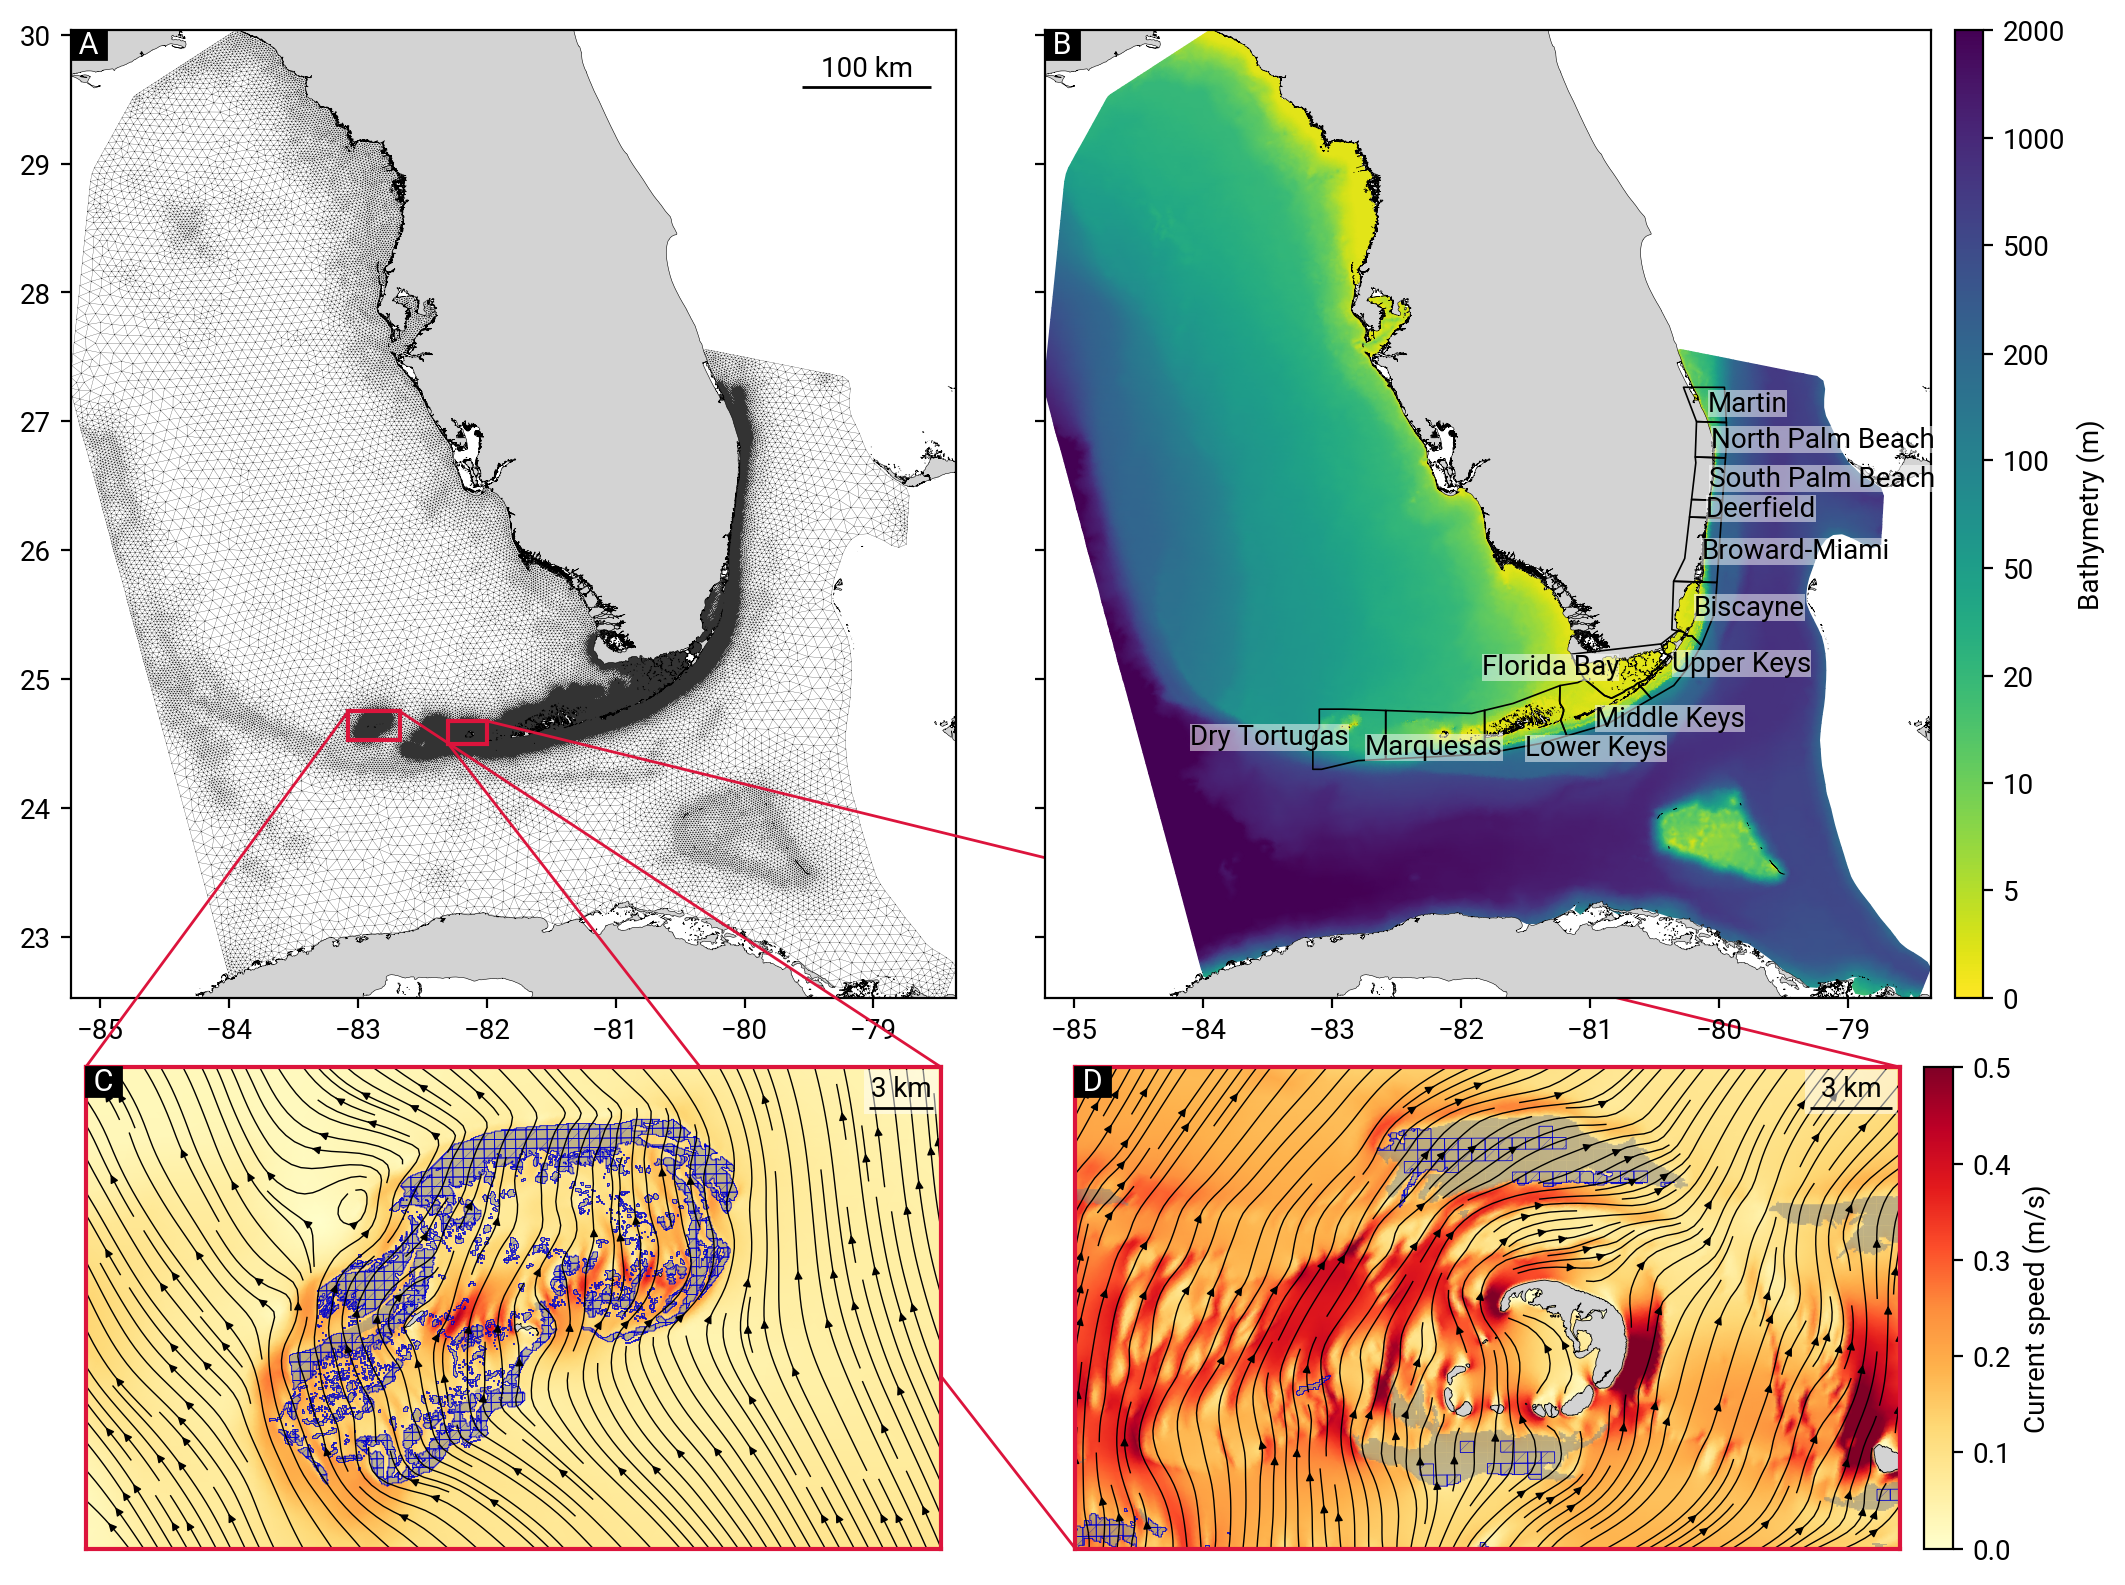
\includegraphics[width=\textwidth]{figures/fig_mesh_tnc.png}
		\caption{Model mesh (\textbf{A}) and bathymetry (\textbf{B}) with close-up views of the simulated currents in the Dry Tortugas (\textbf{C}) and the Marquesas Keys (\textbf{D}). The different regions of Florida's Coral Reef, as defined in the Unified Reef Map are shown in panel (\textbf{B}). This illustrates the ability of the model to capture complex fine-scale flow patterns near reefs and islands. Land is shown in light grey, reefs in dark grey, and reef sub-regions with live corals are represented by blue squares.}
		\label{fig:mesh}
	\end{figure}
	The modeled currents and the experimentally calibrated larval survival and competency parameters were then used to simulate the larval dispersal of \textit{A.~cervicornis}, \textit{C.~natans}, \textit{D.~labyrinthiformis}, \textit{M.~cavernosa}, \textit{O.~faveolata}, and \textit{P.~strigosa}.  Larval dynamics were implemented through mortality and competence, \ie the ability of larvae to settle onto a reef. Mortality was modeled using a Weibull model \citep{king2023larval} with parameters $\lambda$ and $\nu$. After minimum time to competence $t_c$, larvae were becoming competent at a rate $\alpha$ and losing competence at a rate $\beta$ (see \ref{appendix:larvae} for more details). The species-specific spawning dates and times were defined in days after the full moon (DAFM) and minutes after sunset (MAS) \citep{vermeij2021coral}. \textit{D.~labyrinthiformis} spawned in April and May, \textit{M.~cavernosa} in July and August, and all other coral species spawned in August and/or September.
	\pdfcomment[author={Joana Figueiredo},color=green]{I know this is the info I sent you in 2022 because it had been what was reported. The needle of info has moved a bit more now though. We now know that aside from Dlab (after April and/or May moon) and Mcav (after July and August moon), all the others are more after full moon of August and/or September spawners. They can spawn after the July moon but only if the moon is very late in July, often meaning that they spawn already in August, because they spawn about a week later. Not sure what the best way forward is as I understand this affects your simulations. We can always keep it and see if the reviewers notice it. The days of spawn after the full moon still match our knowledge and we are confident on it. For the minutes after sunset (MAS), the best reference is CARMABI tables for spawning predictions for the Southern Caribbean https://www.researchstationcarmabi.org/predictions-for-coral-spawning-events-in-the-southern-caribbean-for-2022/ The actual time they spawn is different from Florida because their sunset occurs at a different time, but the MAS are consistent throughout the Caribbean.. For month of spawning, CARMABI predictions are not good for Florida because at their latitude corals spawn later in the season. There is no published summary of spawning months for Florida. We have just been gathering that information in the latest years, so maybe we can use personal observations.}
	
	The reefs of Florida were extracted from the “coral reefs and hardbottom” layer of the Unified Florida Reef Tract Map \citep{fwc2017unified}. The extracted reef polygon were then further divided into $16,823$ 500 m $\times$ 500 m sub-reef patches to model larval exchanges at a finer scale (Fig. \ref{fig:mesh}). From these $16,823$ polygons, we then excluded any area deeper than 18 meters, or near areas with strong anthropogenic stressors (ports, pipeline corridors, anchorages, etc.), resulting in $10,055$ polygons. More details about the exluded areas can be found in \cite{tnc2024}. We assumed a uniform coral cover over all reefs, and released a total of about $10^6$ particles over all the reef polygons during each spawning simulation. Particles in the model were not representing discrete larvae but rather a continuous amount of larvae, initialized at 1. Settlement of competent larvae onto reef was occurring at deposition rate $\gamma = 0.2$ hour$^{-1}$, consistent with observed larval settling velocity (\citealp{hata2017coral}, Table 1). For each modeled spawning, the exchanges of larval mass between reefs were recorded into connectivity matrices, whose rows correspond to source reefs and whose columns correspond to destination reefs. Connectivity matrices can be more easily interpreted as large networks whose nodes are the reefs and whose edges are the larval exchanges between reefs. Connectivity metrics can then be derived from these networks using graph theory tools. The connectivity indicators used in this study are summarized in Table \ref{tab:indicators}. Finally, we identified reef clusters inside the connectivity networks using the \textit{Strongly Connected Components} (SCC) detection algorithm \citep{nuutila1994finding}. This method groups reefs in the same community if they present numerous bidirectional connections to each other, and if they are weakly connected to reefs located in other clusters. Such methods aim at identifying ecologically separated groups, hence inferring the presence of dispersal barriers between those groups \citep{thomas2014numerical,saint2023biophysical}.
	
	\begin{table}
		\begin{adjustwidth}{-1in}{-1in}
			\centering
			\small
			\begin{tabular}{p{0.25\textwidth}p{0.45\textwidth}p{0.25\textwidth}}
				\hline
				\textbf{Indicator} & \textbf{Description} & \textbf{What it shows} \\
				\hline
				%Weighted connectivity length ($WCL_i$) & $\dfrac{\sum_{j} \tilde{C}_{ij} L_{ij}}{\sum_{j} \tilde{C}_{ij}}$ & Average dispersal distance from origin to destination reef for all particles released over a reef  \\
				Weighted out-degree ($C_\text{out}$) & Weighted combination of the number of reefs to which a given reef sends larvae and the probability of larval export to those reefs & Reef's potential to export larvae \\
				Weighted in-degree ($C_\text{in}$) & Weighted combination of the number of reefs from which a given reef receive larvae and the probability of larval imports from these reefs & Reef's potential to import larvae \\
				Self-recruitment & Proportion of particles settling on a reef that originated from that same reef. & Reef isolation \\
				Local retention & Proportion of particles released on a given reef that settle on the same reef & Self-replenishment potential \\
				Restoration index & $C_\text{out}^{0.8} \times C_\text{in}^{0.2}$ & Reef's potential to export larvae while maintaining its own population \\
				\hline
			\end{tabular}
		\end{adjustwidth}
		\caption{Connectivity indicators used to analyze the dispersal of coral larvae in the reef network.}\label{tab:indicators}
	\end{table}
	
	\subsection*{Connectivity analysis}
	
	We estimated the similarity of the distribution of the connectivity metrics between species using the Pearson correlation coefficient following the methodology described in \cite{boccaletti2014structure}. The correlation was computed between all pairs of simulated species for each indicator of Table \ref{tab:indicators}. The obtained values range from -1 to 1, where 1 indicates a perfect positive correlation, 0 no correlation and -1 a perfect negative correlation.
	
	We identified connectivity hotspots for each indicator across all simulated years and species. For each simulated spawning event, we identified the reefs for which the value of each connectivity indicator was among the top 10\% for that indicator. We then computed the frequency with which each reef was among the top 10\% performers for each indicator across all simulated spawning events. This approach was used for all indicators except self-recruitment. Following the approach of \cite{tnc2024}, we defined our restoration indicator as a weighted geometric average of the weighted in- and out-degrees, in order to identify reefs with the potential to export larvae to other reefs while being sufficiently resilient to maintain their own population. Hotspots of this restoration indicator were identified by evaluating the frequency with which reefs were in the top 10\% performer for this indicator.
	%These species-averaged frequencies can then be multiplied to select optimal restoration sites. Such reef sites could be identified among top performers of weighted out-degree, in-degree and local retention, and low-performers of self-recruitment.
	
	We also assessed the interannual variability of the connectivity indicators and the structure of the communities in the connectivity networks. The variability of the connectivity indicators was computed with the quartile coefficient of dispersion (QCD) of each indicator, for each reef and each simulated species. The QCD is expressed as $(Q_3-Q_1) / (Q_3+Q_1)$, where $Q_1$ and $Q_3$ are the first and third quartiles of the indicator distribution across all simulated spawning events. We then computed the average of the QCD of all species at each reef. Furthermore, we computed the SCCs for each simulated species using the 10 year averaged connectivity matrices. We then computed the SCC using the yearly connectivity matrices to evaluate the variability of the coral communities based on yearly connectivity estimates. This was performed by counting the number of simulated years during which any given pair of reefs was found in the same SCC. This resulted in a symmetric matrix of shape $10,055 \times 10,055$, whose entries ranged between 0 and 10. Entries of this matrix with high values indicate pairs of reefs that were consistently found in the same SCC over the 10 simulated years. Lower values of this indicator for all reef pairs would hence infer a strong interannual variability of the composition of the SCCs.
	
Finally, we assessed the number of simulated years needed to capture the magnitude of the interannual variability of the simulated potential connectivity. This was performed by computing the mean standard deviation of the entries of the yearly species-averaged connectivity matrices as a function of the number of simulated years, following the methodology of \cite{thompson2018variability}. If simulating an additional year increases the mean standard deviation, this would suggest that the number of years simulated so far is not sufficient to capture the interannual variability of the connectivity network. However, if simulating an additional year does not increase the mean standard deviation, this would suggest that the interannual variability of the connectivity network has been sufficiently captured.
	
	% === RESULTS ===
	\section*{Results}
	
	\begin{table}
		\begin{adjustwidth}{-1in}{-1in}
			\centering
			\footnotesize
			\begin{tabular}{lccccccc}
				\hline
				Species & DAFM  & MAS      &  $\lambda$     & $\nu$ & $t_c$  & $\alpha$      & $\beta$ \\
				& [day] & [minute] &  [hour$^{-1}$] & [-]   & [hour] & [hour$^{-1}$] & [hour$^{-1}$] \\
				\hline
				%\textit{A.~cervivornis} & 2 - 4 & 150 - 180 & 0.005123971 & 1.303439 & 156.0769 & 0.008409655 & 0.05612717 \\
				%\textit{C.~natans}      & 6 - 8 & 25 - 115  &  0.005621361 & 1.096544 & 28.20409 & 0.003140281 & 0.04740285 \\
				%\textit{D.~labyrinthiformis} & 10 - 12 & -70 - 10 & 0.006276354 & 1 &  44.99998 & 0.003375632 & 0.01651378 \\
				%\textit{M.~cavernosa}   & 5 - 8 & 15 - 225 & 0.002716095 & 1.49904 & 118 & 0.002647409 & 0.0337848 \\
				%\textit{O. faveolata}   & 5 - 8 & 185 - 255 &  0.004567343 & 1.275355 & 108 & 0.001323208 & 0.04444537 \\
				%\textit{P. strigosa}    & 6 - 8 &  35 - 100, 205 - 270 & 0.007488953 & 1.632956, & 36.01622 & 0.02547463 & 0.1775446 \\
				\textit{A.~cervicornis} & 2 - 4 & 150 - 180 & 0.0051 & 1.30 & 156.1 & 0.0084 & 0.0561 \\
				\textit{C.~natans}      & 6 - 8 & 25 - 115  &  0.0056 & 1.10 & 28.20 & 0.0031 & 0.0474 \\
				\textit{D.~labyrinthiformis} & 10 - 12 & -70 - 10 & 0.0063 & 1.00 &  45.00 & 0.0034 & 0.0165 \\
				\textit{M.~cavernosa}   & 5 - 8 & 15 - 225 & 0.0027 & 1.50 & 118.0 & 0.0026 & 0.0338 \\
				\textit{O. faveolata}   & 5 - 8 & 185 - 255 &  0.0046 & 1.28 & 108.0 & 0.0013 & 0.0444 \\
				\textit{P. strigosa}    & 6 - 8 &  35 - 100, 205 - 270 & 0.0075 & 1.60 & 36.02 & 0.0255 & 0.1775 \\
				\hline
			\end{tabular}
		\end{adjustwidth}
		\caption{Biological and spawning parameters used to simulate the dispersal of larvae for each modeled species: days after the full moon (DAFM), minutes after sunset (MAS), Weibull model parameters for mortality ($\lambda$,$\nu$), minimum time to competence ($t_c$), competence acquisition ($\alpha$) and loss ($\beta$) rates. The mortality rate at larval age $t$ was given by $\lambda\nu(\lambda t)^{\nu-1}$.}\label{tab:species}
	\end{table}
	
	The experimentally calibrated survival and competency parameters are given in Table \ref{tab:species}.  The model of best fit for the shape of mortality of all species was the standard Weibull model except for \textit{D.~labyrinthiformis}, whose mortality was best represented with an exponential model. For all species, the model of best fit for the loss of competency evolution was the exponential model. Best-fitted mortality and competency loss curves are shown against observations in Appendix A (Fig. \ref{fig:mortality} and Fig. \ref{fig:competence}). The rates of larval mortality and acquisition and loss of competency varied among species; however, these differences may not necessarily be species-specific, they are more likely driven by parental history and/or genotype. The main difference between species is the minimum time to pre-competency, i.e. the time it takes embryos to develop into larvae competent to settle and metamorphose. This obligatorily planktonic time is known to be well related to the species egg size \citep{figueiredo2013synthesizing, figueiredo2025predicting}. Among the species studied, \textit{A.~cervicornis} had the longest minimum pre-competency time thus having the highest chances of dispersing away from their natal reef. \textit{Orbicella~faveolata} and \textit{M.~cavernosa} have a pre-competency time of about 6 days, so just 2 days less than \textit{A.~cervicornis}, thus likely still able to disperse long distances. In the other extreme is \textit{P.~strigosa} with a very short pre-competency time and a small competency window. This species should therefore have less chances to disperse and settle closer to their natal reef. Like \textit{P.~strigosa}, the larvae of \textit{D.~labyrinthiformis} and \textit{C.~natans} also have a short pre-competency time, but they remain competent for a longer period of time. Therefore, while a good proportion may self-recruit, they may also be able to disperse longer distances.
	
	
	
	% Indicator Mean correlation    Standard deviation
	% locRet    0.652   0.143
	% wInDeg    0.901   0.054
	% wOutDeg   0.792   0.090
	% selfRec   0.347   0.108
	%
	% Species 1 Species 2   Mean correlation
	% Cnat  Pstr    0.875
	% Mcav  Ofav    0.830
	% Cnat  Ofav    0.754
	% Cnat  Mcav    0.728
	% Acer  Ofav    0.719
	% Acer  Mcav    0.683
	% Acer  Cnat    0.664
	% Cnat  Dlab    0.658
	% Ofav  Pstr    0.643
	% Mcav  Pstr    0.608
	% Dlab  Pstr    0.608
	% Dlab  Ofav    0.599
	% Dlab  Mcav    0.581
	% Acer  Dlab    0.574
	% Acer  Pstr    0.574
	
	Connectivity indicators are more strongly correlated between species with similar spawning windows (Fig. \ref{fig:correlation}). The most strongly correlated indicators were weighted in-degree and out-degree, with a species-averaged correlation factor of $0.901$ and $0.732$ respectively. Local retention, was the least strongly correlated indicator, with an average correlation factor of 0.347. The species pairs with the most strongly correlated connectivity were \textit{C.~natans} and \textit{P.~strigosa}, and \textit{M.~cavernosa} and \textit{O. faveolata}, with an average correlation factor of 0.88 and 0.83, respectively, across all considered indicators. These two pairs of species have similar spawning windows and time to competence (Table. \ref{tab:species}). However, the connectivity of \textit{D.~labyrinthiformis}, which spawns in April-May, was more weakly correlated with the other species, which spawn in July-August. Our result also suggest that the duration of the daily spawning (in MAS) is a significant driver of the correlation between connectivity indicators. As the species with the widest daily spawning windows in terms of MAS, \textit{P. strigosa} tended to be more weakly correlated with most other species spawning during the same months with narrower windows. It was most weakly correlated with \textit{A. cervicornis}, which exhibited the narrowest spawning window in terms of MAS.
	% Nevertheless, \textit{A.~cervicornis}. and \textit{P.~strigosa} had the most weakly correlated connectivity indicators, with an average correlation coefficient of 0.574. This might be explained by the fact that \textit{A.~cervicornis} had the narrowest spawning window in terms of MAS, and \textit{P.~strigosa} the widest.
	
	
	\begin{figure}
		\centering
		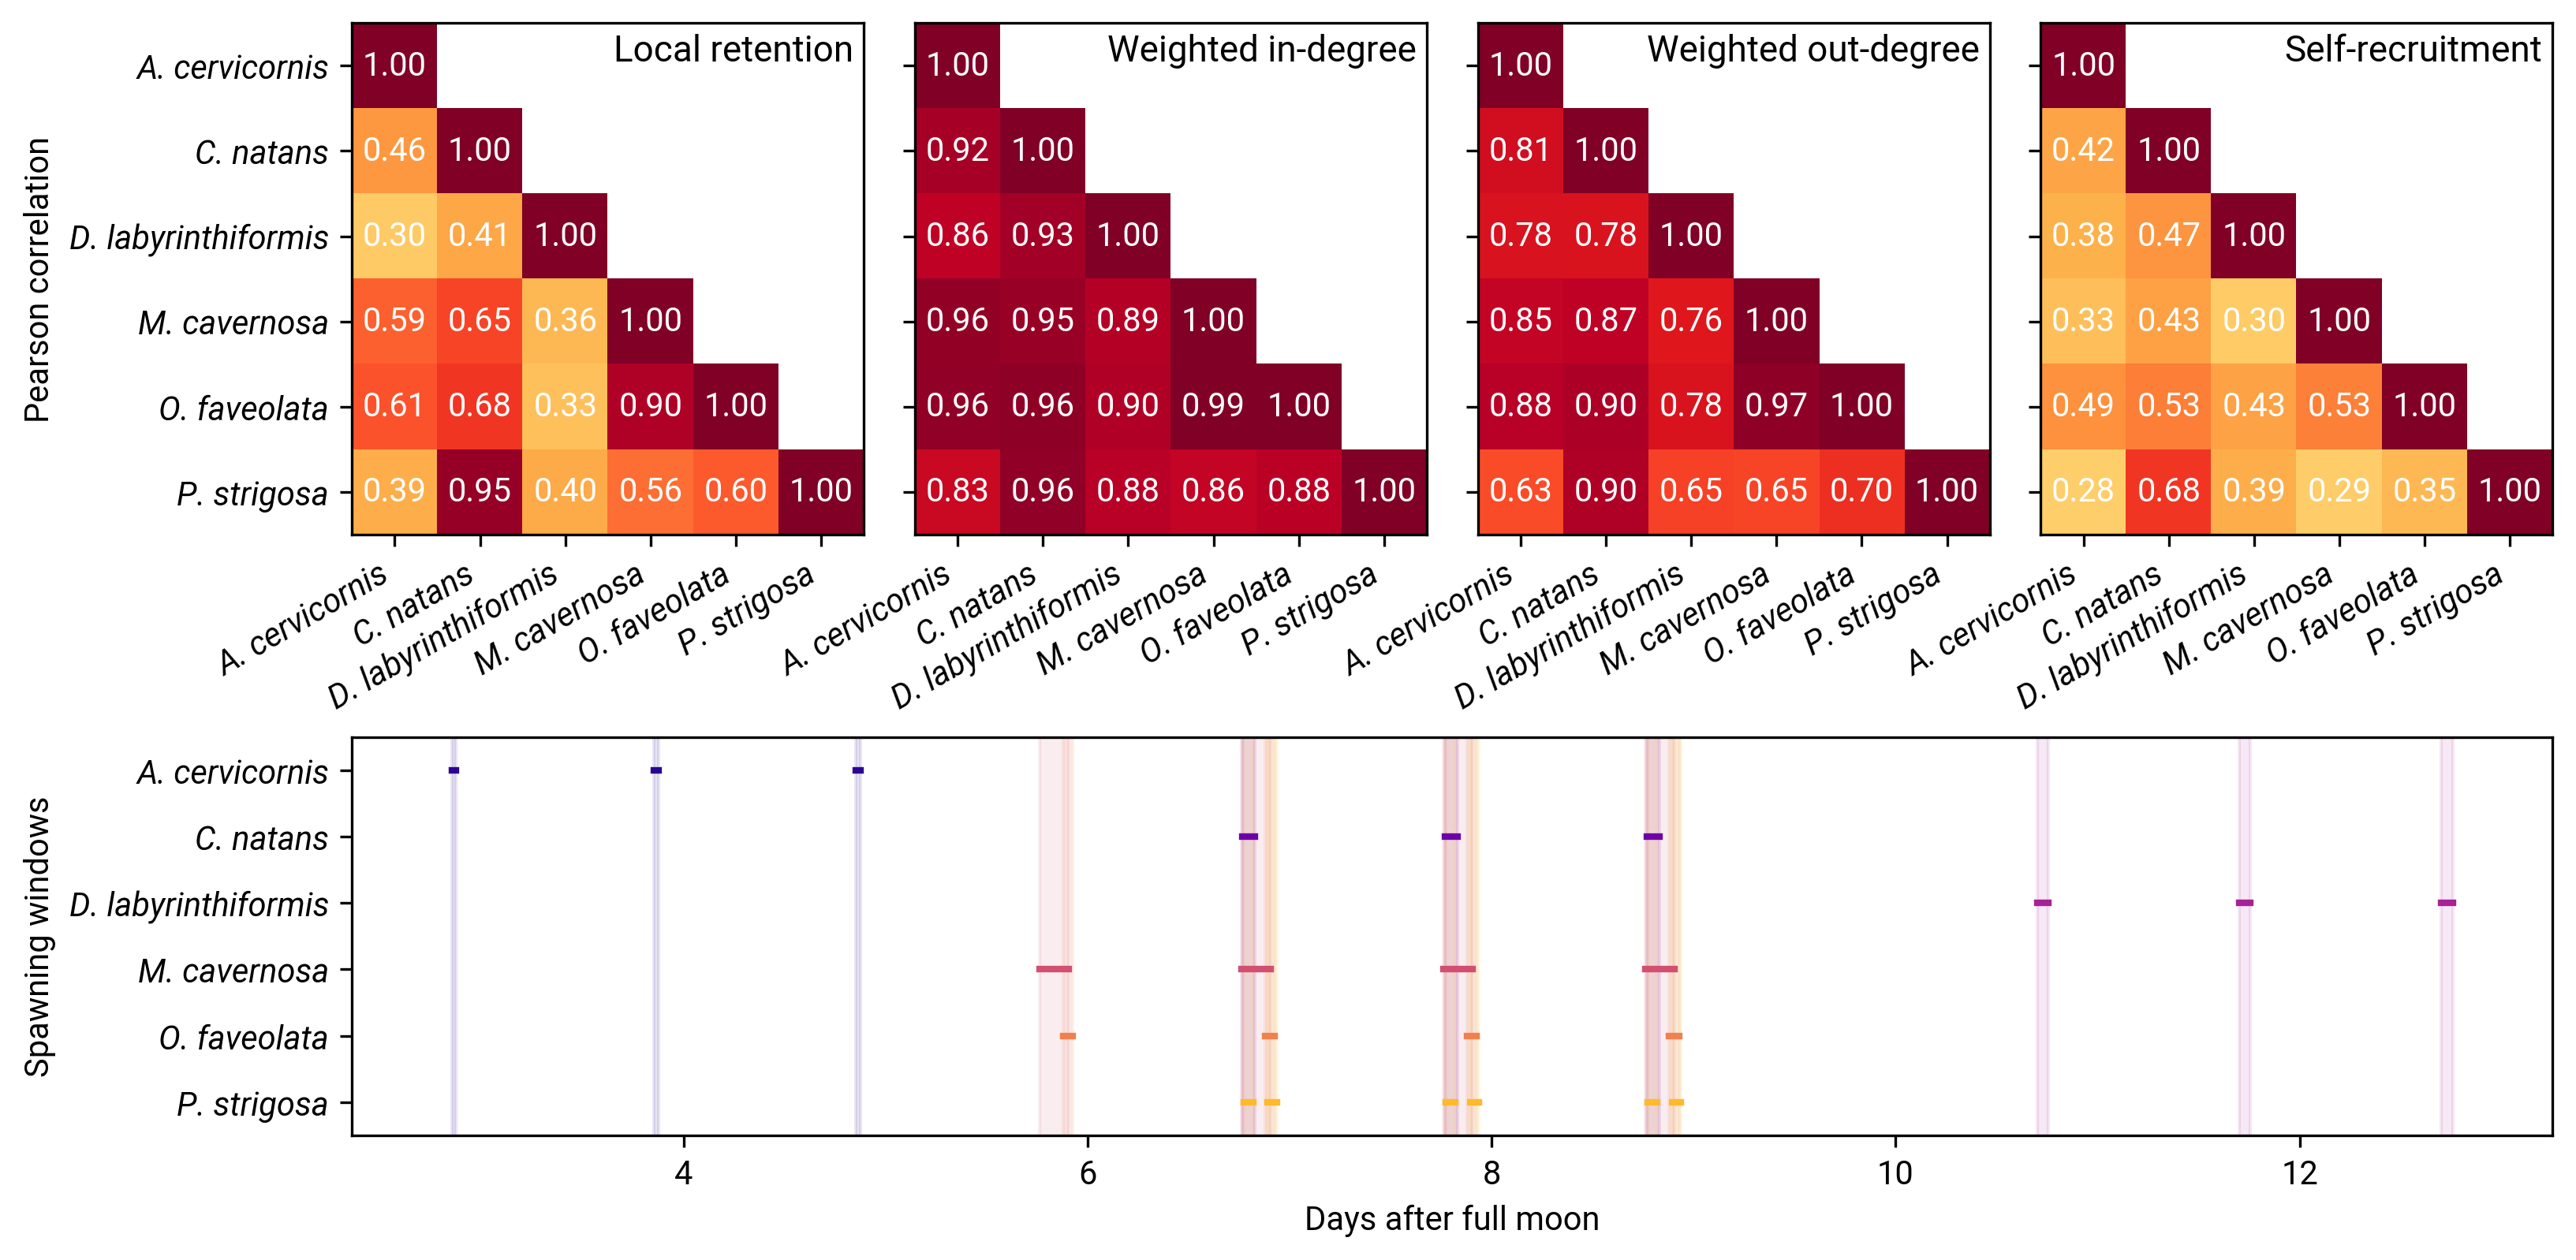
\includegraphics[width=\textwidth]{figures/fig_correlation.png}
		\caption{\textbf{Top}: Pearson correlations of the distributions of local retention, weighted in-degree and out-degree, and self-recruitment for all pairs of species. \textbf{Bottom}: Spawning windows of all coral species in days after full moon. Note that \textit{D.~labyrinthiformis} spawns in April-May, while all other species spawn in July-August. Connectivity indicators are more strongly correlated between species with similar spawning windows.}\label{fig:correlation}
	\end{figure}
	
	When looking at the spatial distribution of the different connectivity indicators, we can identify clusters of top-performing reefs (Fig. \ref{fig:top10}). For local retention, they were found in the Dry Tortugas, north of the Marquesas, in the Upper Keys, and in the northern Broward-Miami and Deerfield. Top performers in terms of weighted in-degree were found in the northern FCR (above latitude 25.6) and in the Dry Tortugas. Top-performers in terms of weighted out-degree were found in the Dry Tortugas, Biscayne, Broward-Miami regions. The presence of reefs with high out-degrees (\ie good sources) in the Dry Tortugas and high in-degrees (\ie good sinks) north of Biscayne suggests that larval exchanges are mostly driven northward by the Florida Current. However, the clusters of reefs with high local retention (\ie high ability to self-replenish) and in-degree in the Dry Tortugas indicate that this northward transport may be disrupted, causing larval retention in the Dry Tortugas.
	
	As the weighted in- and out-degrees are the two indicators with the best defined clusters to top performing reefs, we combine them to build a restoration indicator. Following the approach of \cite{frys2020fine}, we assume that a reef well suited for restoration efforts should, at the same time, be a good source reef (to have a positive impact on reefs downstream) and also a good sink reef (to bolster its resilience against disturbances). Following the approach of \cite{tnc2024}, we consider a weighted geometric average of both indicators with exponents of 0.8 for the out-degree and 0.2 for the in-degree, \ie $R = C_\text{out}^{0.8} \times C_\text{in}^{0.2}$. The resulting indicator shows that reefs with the greatest restoration potential are mostly located the Dry Tortugas and northern Broward-Miami, and more marginally in the Middle Keys and North and South Palm Beach (Fig. \ref{fig:top10}).
	
	\begin{figure}
		\centering
		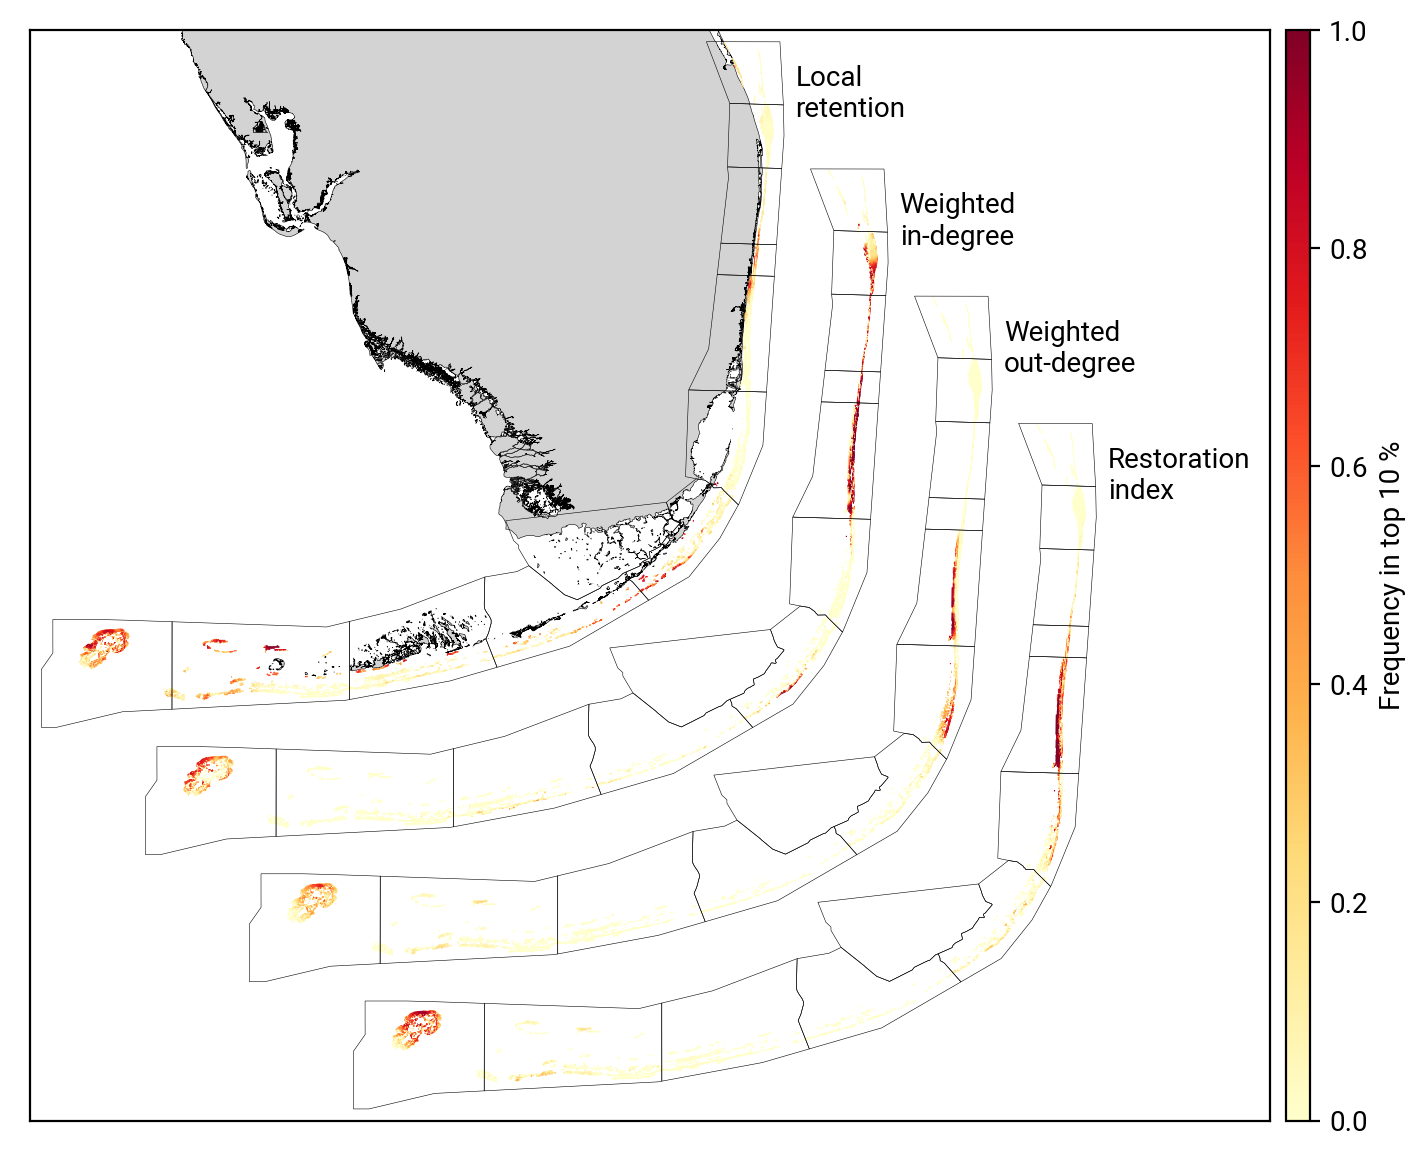
\includegraphics[width=0.95\textwidth]{figures/fig_top10.png}
		\caption{Frequency of reefs in the top 10\% performers for local retention, weighted in-degree, weighted out-degree and restoration index. The restoration index was computed as weighted geometric average of the weighted in- and out-degrees. Clusters of top performers were found in the Dry Tortugas for all indicators. Other clusters of top-performers were found in Biscayne and Broward-Miami for weighted out-degree, and north of Biscayne for weighted in-degree. Clusters of top-performers were more spread out across the whole FCR for local retention.}\label{fig:top10}
	\end{figure}
	
	Self-recruitment exhibited the highest interannual variability, as indicated by large quartile coefficients of dispersion across most reefs (Fig. \ref{fig:variability}). This would suggest that no reef is continuously isolated over time in the network. Local retention also displayed significant interannual variability, except in the Marquesas, Biscayne, and North Palm Beach regions, where smaller quartile coefficients of dispersion were observed. In contrast, weighted in- and out-degrees were relatively stable across most reefs, with some exceptions. Significant variability in both indicators was detected in the Dry Tortugas and Lower Keys, primarily on the outer shelf. Additionally, the weighted out-degree exhibited larger variability in the northernmost part of the FCR, particularly in North Palm Beach and the Lower Keys. These patterns suggest that, while in- and out-degrees remain mostly consistent over time, they can still fluctuate in areas where the ocean circulation is more variable, \ie on the outer shelf and between the Dry Tortugas and the Lower Key. Local retention and self-recruitment are subject to more widespread interannual fluctuations. Computing the  quartile coefficient of dispersion (QCD) using all connectivity matrices gives similar results for the weighted in- and out-degrees, but QCDs close to 1 on all reefs for local retention and self-recruitment. This indicates that the latter two indicators show significant interspecific variability while weighted in- and out-degrees are more uniform across species.
	
	\begin{figure}
		\centering
		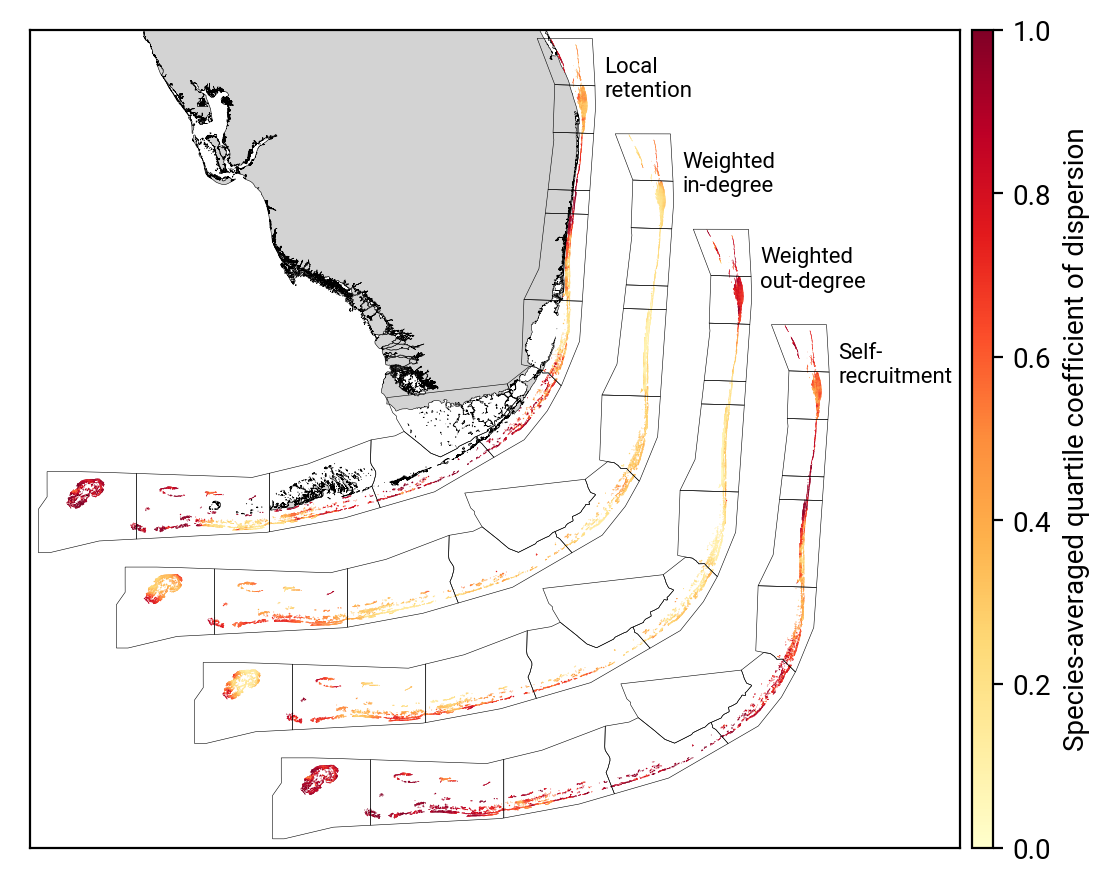
\includegraphics[width=\textwidth]{figures/species_averaged_quartile_coefficient_of_dispersion.png}
		\caption{Interannual variability of the species-averaged connectivity indicators as measured with the quartile coefficient of dispersion. Weighted in- and out-degrees only exhibited significant interannual variability in some parts of FCR, while significant interannual variability in terms of local retention and self-recruitment was observed on most reefs.
			%			\pdfcomment[color=yellow]{
				%				Key messages:\textCR
				%				* In- and out-degrees are rather stable with the exception of the Dry Tortugas and Lower Keys (mostly on the outer shelf) for both indicators, and the nothermost part of the FCR for the weighted out-degree\textCR
				%				\textHT - For variability of DT, mention retention of particles on the WFS in the discussion $\Rightarrow$ prevents long-distance dispersal of larvae from the DT (larval retention due to eddies observed in other papers)\textCR
				%				* Local retention and self-recruitment have much more spreadout interannual variability
				%			}
		}\label{fig:variability}
		
	\end{figure}
	
	Given the interannual variability in ocean circulation patterns within and around the FCR, and the resulting fluctuations in potential connectivity, we evaluated the number of simulated years required to accurately capture the observed magnitude of interannual potential connectivity variability over the 10-year simulation period. We find that connectivity variability increases with simulation length up to approximately 8 years, after which it stabilizes near the mean value observed in the full 10-year simulation (Fig. \ref{fig:saturation}). These findings indicate that a simulation length of at least 8 years is necessary to capture more than 96\% of the total (intra-annual and interannual) potential connectivity variability (Fig. \ref{fig:saturation}). Additionally, simulations shorter than 5 years account for, at most, 80\% of the total variability, potentially leading to an incomplete understanding of stability in connectivity.
	
	\begin{figure}
		\centering
		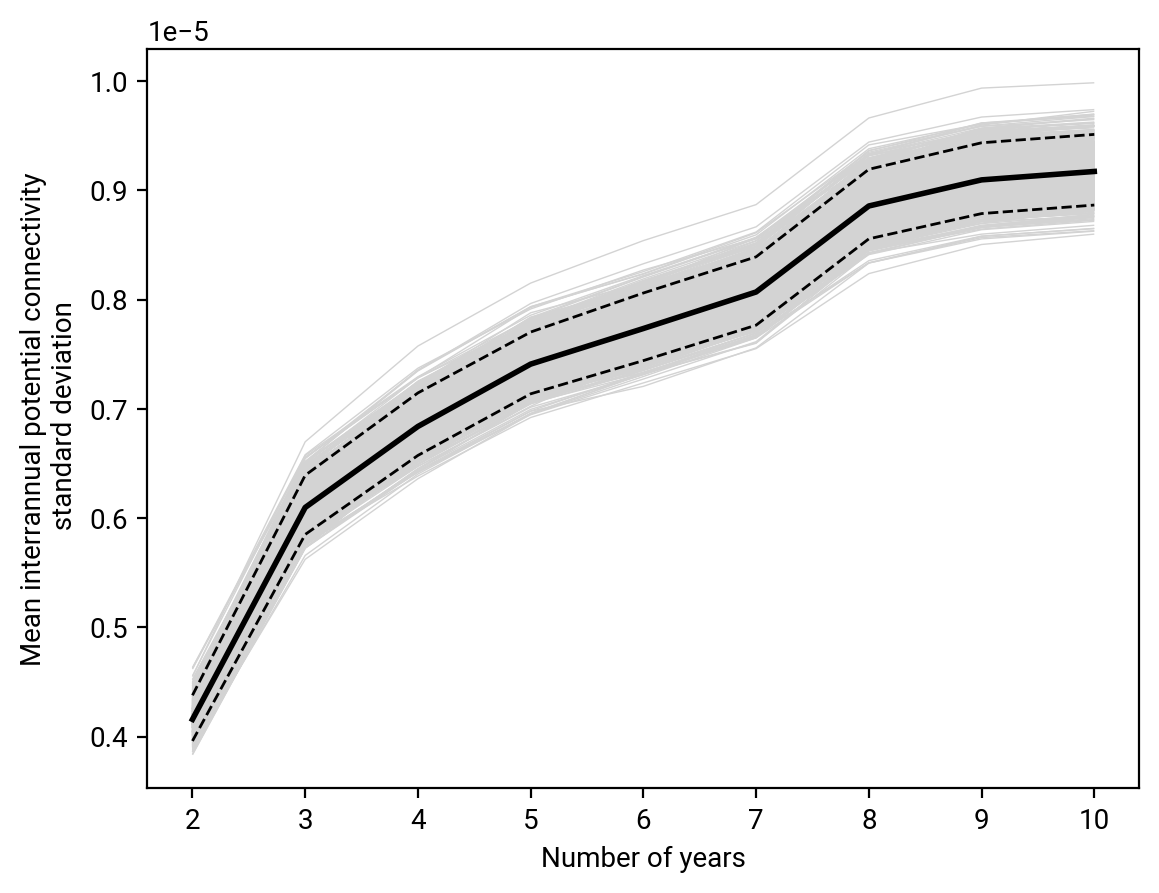
\includegraphics[width=0.8\textwidth]{figures/fig_cm_std.png}
		\caption{Mean interannual potential connectivity standard deviation (the average standard deviation of annual mean potential connectivity across all source-sink site combinations) as a function of the number of years over which potential connectivity was simulated (black line). Dashed black lines represent the 5th and 95th percentiles of 1000 random realizations (gray), where the (annual) temporal sequence was randomly sampled from the potential connectivity simulation. These results indicate that a simulation length of at least 8 years is necessary to capture more than 96\% of the total (intra-annual and interannual) potential connectivity variability}\label{fig:saturation}
	\end{figure}
	
	A Strongly Connected Component (SCC) was found in the Dry Tortugas for all simulated species using the 10-year-averaged connectivity networks (Fig. \ref{fig:scc}). Large communities were also found in the Florida Keys for all species except \textit{O.~faveolata}, which exhibited the most fragmented SCCs. However, \textit{D.~labyrinthiformis} exhibited a large SCC covering the entirety of the Florida Keys. Additionally, large SCCs were found between Deerfield and North Palm Beach for all species except \textit{O.~favelolata}, with \textit{C.~natans} and \textit{P.~strigosa} exhibiting the largest communities in this area. Our results suggests that the SCC in the Dry Tortugas was stable for all species, with most pairs of reefs in the Dry Tortugas found in the same SCC for most simulated years. Stable communities were also found in the Upper Keys, and Deerfield and South Palm Beach for most species. \textit{D.~labyrinthiformis} exhibited the largest, most stable communities, with large groups of reef pairs found in the same SCC in the Dry Tortugas, the Marquesas, and the Keys. Our results suggest that SCCs of \textit{A.~cervicornis} in the Keys were unstable as numerous reef pairs in this area were found in the same SCC during at most 2 years. \textit{P.~strigosa} and  \textit{O.~faveolata} exhibited a more local community structure, as SCCs were mostly made of reef pairs from the same region.

	% Finally, we assessed the structure and composition of the SCCs evolved through time for each simulated species (Fig. \ref{fig:scc}). \textit{A.~cervicornis}, \textit{M.~cavernosa} and \textit{O.~faveolata} exhibited the least stable SCC structure, as they yield the weakest number of reef pairs found in the same SCC during all 10 simulated years, with \textit{O.~faveolata} having the least stable SCC structure \pdfcomment[color=orange,author=Dan]{I struggle with this interpretation! An SCC is necessarilly a multi-generational structure. Shouldn't it be estimated over the 10 year matrix? Is a larger but "weaker" SCC better or worse than a smaller more "stable" one?}. The largest number of reef pairs found in the same SCC during all 10 simulated years was observed in the connectivity network of \textit{D.~labyrinthiformis}, suggesting that this species had the most stable connectivity networks. A comparison of the SCC composition of \textit{O.~faveolata} and \textit{D.~labyrinthiformis} in 2017 and 2018 is shown in Fig. \ref{fig:scc}. While most of the SCC structure is conserved between those two years for \textit{D.~labyrinthiformis}, strong structural differences are observed for \textit{O.~faveolata}, especially in the Middle Keys and the Dry Tortugas. Nonetheless, some reefs were consistently found in the same communities for all simulated species and years. These reefs are located in the northern Dry Tortugas, north of the Marquesas, and in the Upper Keys (Fig. \ref{fig:mean_counter}).
	
	
	\begin{figure}
		\centering
		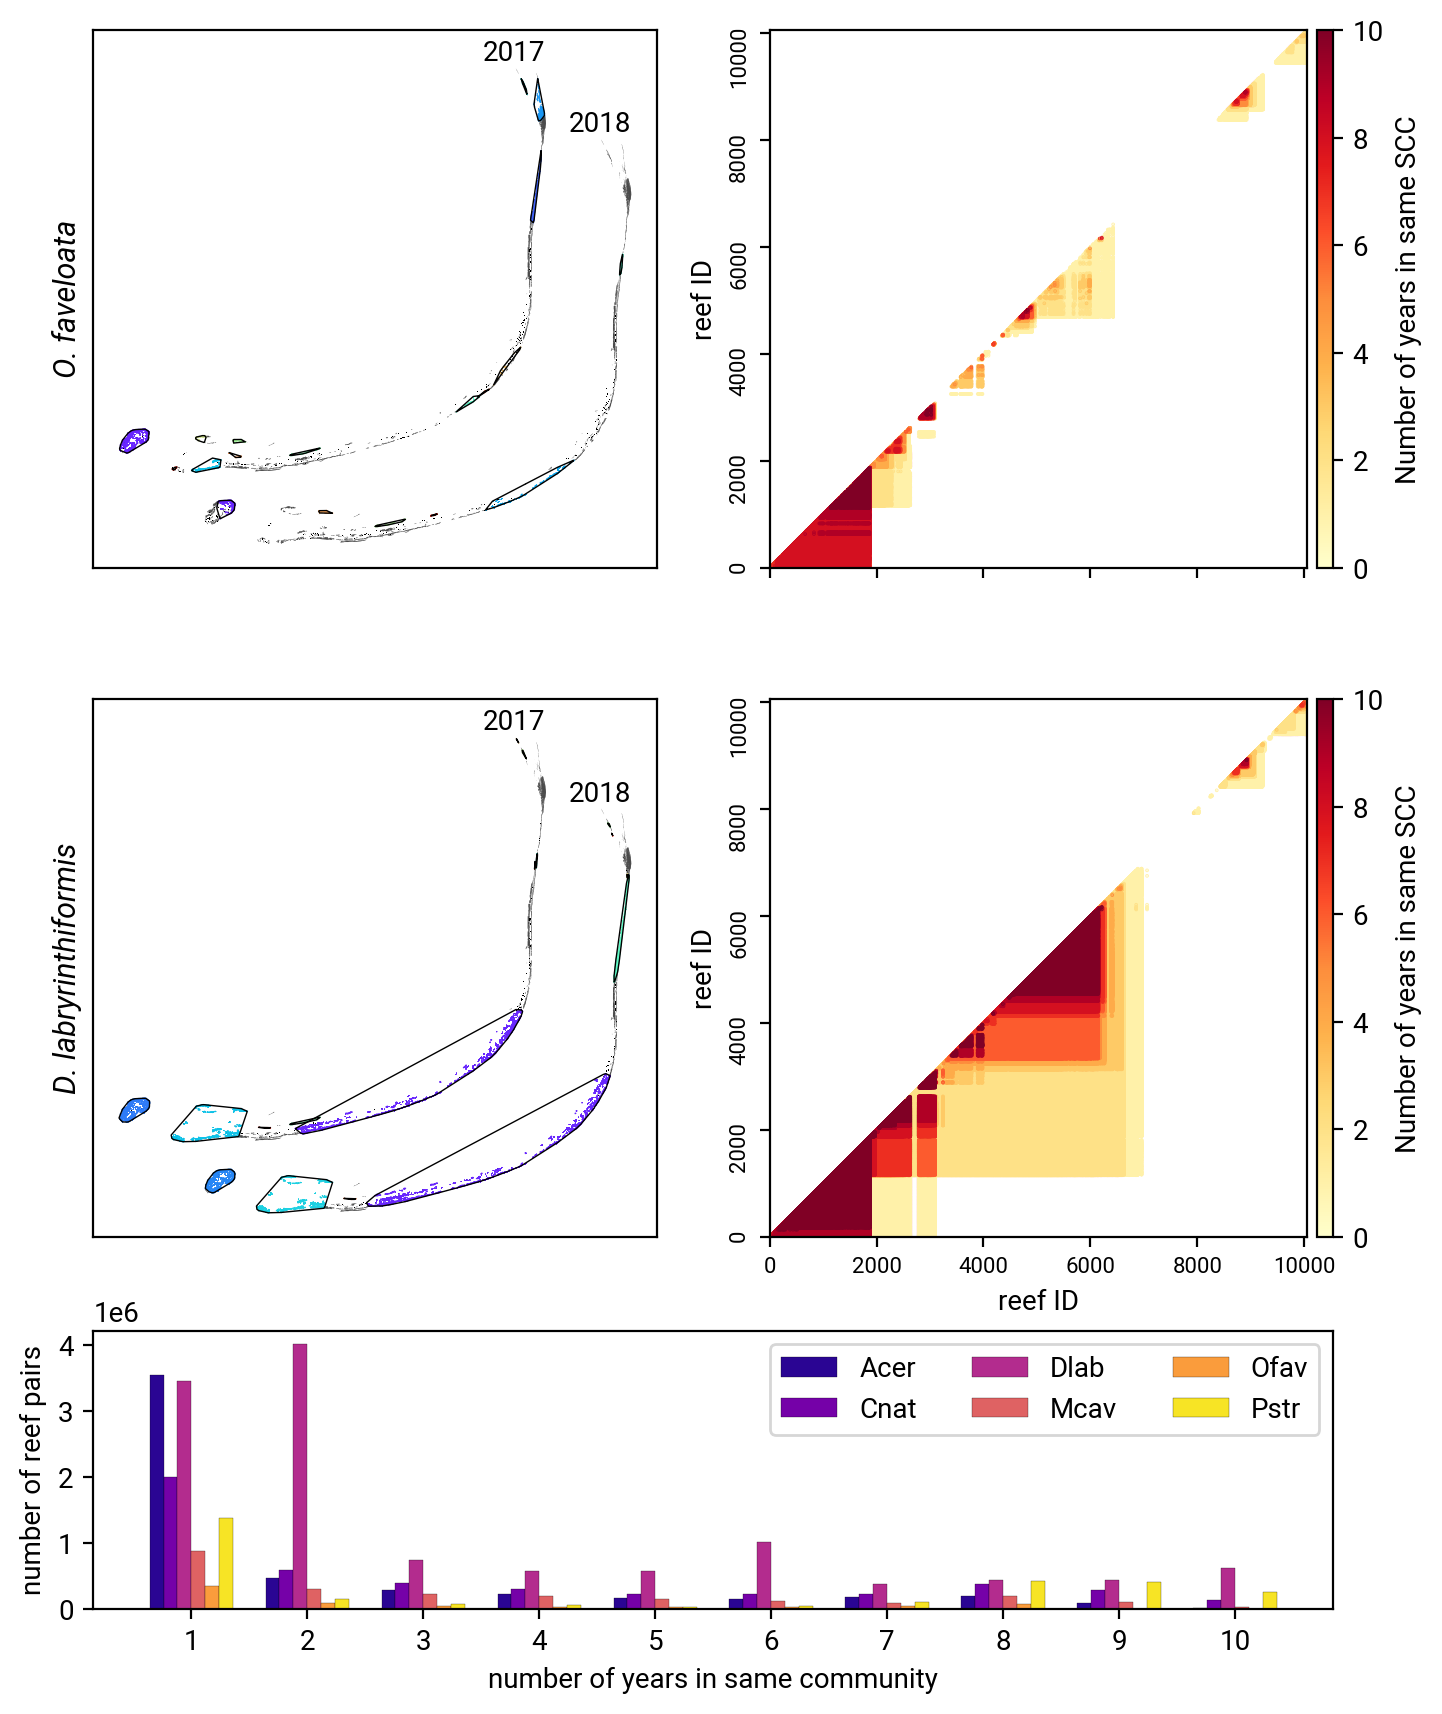
\includegraphics[width=.98\textwidth]{figures/comparison_sccs.png}
		\caption{Strongly Connected Components (SCCs) derived from the 10-year-averaged connectivity networks of all species (\textbf{top left}). The other panes show the lower parts of the symmetrical matrices indicating the number of simulated years during which each pair of reefs was found in the same SCC for these all species. Reefs are ordered according to their geographical coordinates. Reefs of the bottom left (resp. top right) of the matrix correspond to reefs located in the south-west (resp. north east) of FCR. The delimitation of the regions of FCR is shown by gray lines. Regions 8, 9 and 11 were not added to the panes for readability reasons. For all species, a SCC is found in the Dry Tortugas, while the SCCs of the Florida Keys tend to be more variable across species.}\label{fig:scc}
	\end{figure}
	
	% === DISCUSSION ===
	
	\section*{Discussion}
	
	% §1 : Summary of take-home messages
	In this study, we combined experimental measurements of coral larval traits with biophysical modeling to assess the potential connectivity of six key reef-building coral species in the Florida Coral Reef (FCR) over a 10-year period. Effective biophysical connectivity studies require high-quality experimental data to characterize the coral larvae's biological traits, which directly influence the duration during which larvae can drift before settling on a reef, and sufficiently long, fine-scale hydrodynamic simulations to capture both interannual oceanic variability and the scale of individual reefs. Our results show that connectivity indicators for coral species with similar spawning windows are strongly correlated, making such "correlated species" suitable candidates for joint restoration efforts. This is evident, for instance, in the cases of \textit{P.~strigosa} and \textit{C.~natans}, as well as \textit{M.~cavernosa} and \textit{O.~faveolata}. The weighted in- and out-degree indicators reveal stable clusters of reefs that consistently perform well across all species and throughout the simulation period. In contrast to self-recruitment and local retention, source and sink indicators exhibited limited interannual variability, reinforcing their utility in identifying reefs with strong restoration potential. Additionally, the stability of reef communities over time varies significantly between species; some species form smaller, less stable communities, suggesting the need for more localized and short-term management strategies.
	
	% § 2 : Importance of ocean currents in shaping connectivity variability
	Connectivity is shaped by the interplay between the ocean circulation and the coral larvae biological traits. The ocean circulation patterns around coral reefs in Florida are primarily driven by the Florida Current (FC), which flows from southwest to northeast and facilitates long-distance larval transport along the outer shelf. The meandering of the FC and its associated eddies modulate these connectivity pathways \citep{lee1994evolution,kourafalou2012florida}. In contrast, circulation on the inner shelf is largely governed by local winds and tides, resulting in more localized and predictable transport patterns \citep{lee2002volume,liu2012seasonal}. On the inner shelf, currents exhibit a well-defined seasonal cycle, which can either enhance or restrict larval dispersal depending on the timing of spawning events \citep{liu2012seasonal}. In contrast, the outer shelf, dominated by the FC, shows limited seasonality but significant interannual variability, primarily due to the influence of Loop Current (LC) eddy separation events \citep{kourafalou2012florida}. These eddy events can modify the path and intensity of the FC, intermittently creating or obstructing connectivity pathways along the Florida's Coral Reef. The region between the Dry Tortugas and the Marquesas presents a particularly complex case due to the influence of mesoscale eddies, especially the Tortugas eddies \citep{dobbelaere2022connecting}. These eddies can remain stationary near the Dry Tortugas for up to 120 days, effectively disrupting westward larval transport from the Marquesas and acting as barriers to connectivity \citep{fratantoni1998influence,kourafalou2012florida}. Connectivity between these regions lacks a clear seasonal pattern and exhibits high interannual variability, likely due to the unpredictable presence of these eddies and variations in LC penetration \citep{lee1994evolution}.
	
	% § 3 : Biological aspects explaining interspecific variability
	% -> Add differences in spawning windows to the paragraph
	The variability induced by ocean circulation is further compounded by biological variability among coral species. Most species spawn in July–August, typically between 2 and 12 days after the full moon, except for \textit{D.~labyrinthiformis}, which spawns in April–May. Larvae released at different spawning times encounter distinct oceanic conditions, resulting in varying dispersal pathways. This temporal difference in spawning likely explains the weaker correlation observed between connectivity indicators for species with widely separated or narrow spawning windows. The interspecific variability in larval survival and competency dynamics also explains the interspecific variability in connectivity patterns. For all species, larval survival decreased over time for all species (Fig. \ref{fig:mortality}) because coral larvae are mainly lecithotrophic and thus their energy reserves slowly become exhausted resulting in eventual death. It remains to be determined if the recorded rates of larval mortality are species-specific and/or driven by parental genotype, history of stress exposure, food quantity and quality they had access to, and/or symbiont community \citep{jones2011tradeoffs, baums2013genotypic, padilla2013all, kirk2018genomic}. The estimated rates of acquisition (a) and loss of competency (b) also differed between species (Table \ref{tab:species}). For some species, the proportion of larvae that settled was quite low (Fig. \ref{fig:top10}), thus is possible that the crustose coralline algae and microbial biofilm used to induce settlement were not as adequate for them. However, the species that displayed lower settlement, \textit{P.~strigosa}, also registered the highest mortality suggesting that rather than species-specific, rates of mortality, and acquisition and loss of competency are mostly explained by parental condition. The interspecific differences in the minimum time to competency are unequivocally species-specific, and mostly explained by their egg size \citep{figueiredo2013synthesizing, figueiredo2025predicting}. As egg size (and ratio of the surface-area to the volume) increases, the elimination of CO$_2$ (which is toxic) from the embryo surface is progressively harder, reducing the pace of larval development \citep{berrill1935cell, einum2002egg}.
	
	% § 4 : There are clusters of reefs that are consistently good sources and good sinks and are hence well suited to derive restoration or conservation metrics:
	\modif{We identified reefs with strong restoration potential in regions including the Dry Tortugas and northern Broward-Miami, and to a lesser extent, the Middle Keys and North and South Palm Beach. These were identified using a restoration index defined as a weighted geometric mean of source and sink indicators}. Identifying clusters of reefs consistently acting as good sources or sinks of larvae is essential for developing effective restoration and conservation strategies. The interannual variability of weighted in- and out-degree connectivity indices -- proxies for sink and source characteristics -- is limited for most reefs, suggesting that management planning based on these connectivity metrics will be robust. Local retention (a measure of self-persistence) and self-recruitment (indicating reef isolation) show greater variability across years, hence limiting their use for reef management. Reefs characterized by high source indices should be prioritized for restoration and protection due to their significant downstream footprint. Such reefs are also good places to establish spawning hubs, \ie areas where corals from different sites are moved to a smaller area to be in close proximity and thus, when they spawn, maximize chances of successful fertilization. Conversely, reefs with higher sink indices, while less valuable for active restoration, play a critical role as reservoirs of genetic diversity. They support network persistence and represent valuable sites for donor fragment collection for nurseries or outplanting \citep{king2023larval}. Furthermore, reefs exhibiting relatively high values in both source and sink indices can act as stepping stones for multigenerational connectivity, receiving larvae from many reefs and subsequently distributing larvae widely \citep{frys2020fine}. Such reefs contribute substantially to maintaining network-wide genetic diversity and resilience, making them high-priority candidates for both protection and restoration efforts.
	
	
	% \modif{We identified reefs with strong restoration potential in regions including the Dry Tortugas and northern Broward-Miami, and to a lesser extent, the Middle Keys and North and South Palm Beach}. We used a restoration index defined as a weighted geometric of source and sink indicators, emphasizing the source component to highlight reefs with significant contributions to network resilience and downstream connectivity. However, we also incorporated a sink component, albeit with a smaller weight, to ensure selected reefs possess sufficient resilience to withstand and recover from disturbances such as bleaching events, coral disease outbreaks, or hurricanes.
	
	% § 6
	\modif{We found stable strongly connected components (SCC) in the Dry Tortugas and the Upper Keys. These are groups of reefs presenting numerous bidirectional connections.} Restoring reefs found within large and stable community should thus have durable effects on the other reefs of the community. Although the interannual variability of the community composition and structure varied across species, some groups of reefs were consistently found in the same SCC for all simulated years and species. The largest of these invariant components were found in the northern Dry Tortugas, the northern Marquesas, and the Upper Keys. Except for the Upper Keys, these regions correspond to sheltered inshore areas that are less affected by the variability of the outer-shelf circulation. Our results suggest that the interspecific variability of the SCC structure was partly driven by the biological traits of the coral larvae. Species with low precompetency period and high mortality such \textit{D.~labyrinthiformis} and \textit{P.~strigosa} tended to have more reef pairs in the same SCC for all simulated years. The connectivity of such species is dominated by shorter-distance connections \citep{figueiredo2022global}. As larvae settle sooner and closer from their reef of origin, their dispersal is less likely to be impacted by the variability of the outer-shelf ocean circulation.
	
	
	% § 7 : Limitations of this study
	Although the use of a 2D model made estimating coral connectivity across a large number of years and species computationally tractable, it also implied modeling assumptions and limitations. Coupling \slim with \hycom allowed the model to capture baroclinic features such as mesoscale eddies near the Dry Tortugas \citep{dobbelaere2022connecting}. However, due to its barotropic nature, \slim might be underestimating submesoscale eddy activity along the Florida shelf. This underestimation of current variability might lead to an overestimation of the "conveyor belt effect" of the Florida Current \citep{frys2020fine} and an underestimation of local larval retention. However, the recent developments in GPU-accelerated ocean models may make the use of high-resolution 3D barotropic model computationally feasible for this type of long-term study in the near future. Computational costs would then be especially critical as more simulated years are expected to be needed to capture the interannual variability of such models. Furthermore, this study relied on potential connectivity, as we assumed a uniform coral cover over all reefs and did not account for habitat suitability and post-settlement survival. Successful coral settlement may indeed be impeded by various factors such as soundscape \cite{lillis2016variation}, substrate characteristics \citep{jorissen2021coral} or competition with turf algae and macroalgae \cite{webster2015macroalgae}. Taking these factors into account, the potential connectivity matrices computed in this study might then be further refined into effective connectivity matrices by pre- and post-multiplying them by habitat suitability matrices.
	
	
	% § 8 : General conclusions and perspectives
	% -> Add disease risk as negative cnnectivity component?
	By combining a high-resolution ocean model with lab experiments, we evaluated the connectivity of 6 coral species over a period long enough to capture the variability in ocean circulation. Based on this long-term connectivity, we derived robust indicators to inform coral restoration strategies beneficial to all species considered, \modif{and identified reefs with high string restoration potential in the Dry Tortugas and northern Broward-Miami}. In a context of rapidly declining coral populations, this study provides additional tools to optimize the selection of restoration sites to ensure durable and widespread impacts. The presented indicators could be further refined by incorporating data about coral cover, water and habitat quality, and disease connectivity to account for the risk of coral bleaching or infection by stony coral tissue loss disease.
	
	% === Lots of stuff ===
	
	\section*{Data availability}
	
	TBD.
	% The datasets generated during the current study are available from the corresponding author on reasonable request.
	
	\section*{Code availability}
	
	The \slim source code can be found at \href{https://git.immc.ucl.ac.be/slim/slim}{https://git.immc.ucl.ac.be/slim/slim}.
	
	\section*{Acknowledgements}
	
	Computational resources have been provided by the supercomputing facilities of the \textit{Universit\'e catholique de Louvain} (CISM/UCLouvain) and the \textit{Consortium des \'Equipements de Calcul Intensif en F\'ed\'eration Wallonie Bruxelles} (CECI) funded by the \textit{Fonds de la Recherche Scientifique de Belgique} (F.R.S.-FNRS) under convention 2.5020.11. Thomas Dobbelaere is a postdoctoral researcher supported by the F.R.S-FNRS. Florida Department of Environmental Protection for research funds awarded to J.F., MSC Foundation for scholarship awarded to R.C., University of North Carolina Wilmington and Florida Aquarium’s Center for Conservation for the donation of larvae, and all members of the NSU’ Marine Larval Ecology and Recruitment lab for assistance. Activities were conducted under the Florida Fish and Wildlife permit SAL-22-2238A-SCRP.
	
	\section*{Author contributions statement}
	
	TBD.
	
	\section*{Competing interests}
	
	The authors declare no competing interests.
	
	%  === REFERENCE ===
	
	\bibliographystyle{elsarticle-harv}
	\bibliography{biblio.bib}
	\newpage
	
	
	% === APPENDIX === %
	\appendix
	\setcounter{figure}{0}
	\setcounter{table}{0}
	
	% === Invariant component of the SCCs === %
	\section{Invariant component of the SCCs}
	
	We computed the number of years that each pair of reefs was found in the same strongly connected component (SCC) for all simulated species. This indicator was then species-averaged. Reef pairs with a species-averaged indicator value of 10 would thus correspond to pairs of reefs that were found in the same SCC for all computed connectivity networks. The largest robust reef communities were found in the northern Dry Tortugas, north of the Marquesas, and in the Upper Keys.
	
	\begin{figure}[h!]
		\centering
		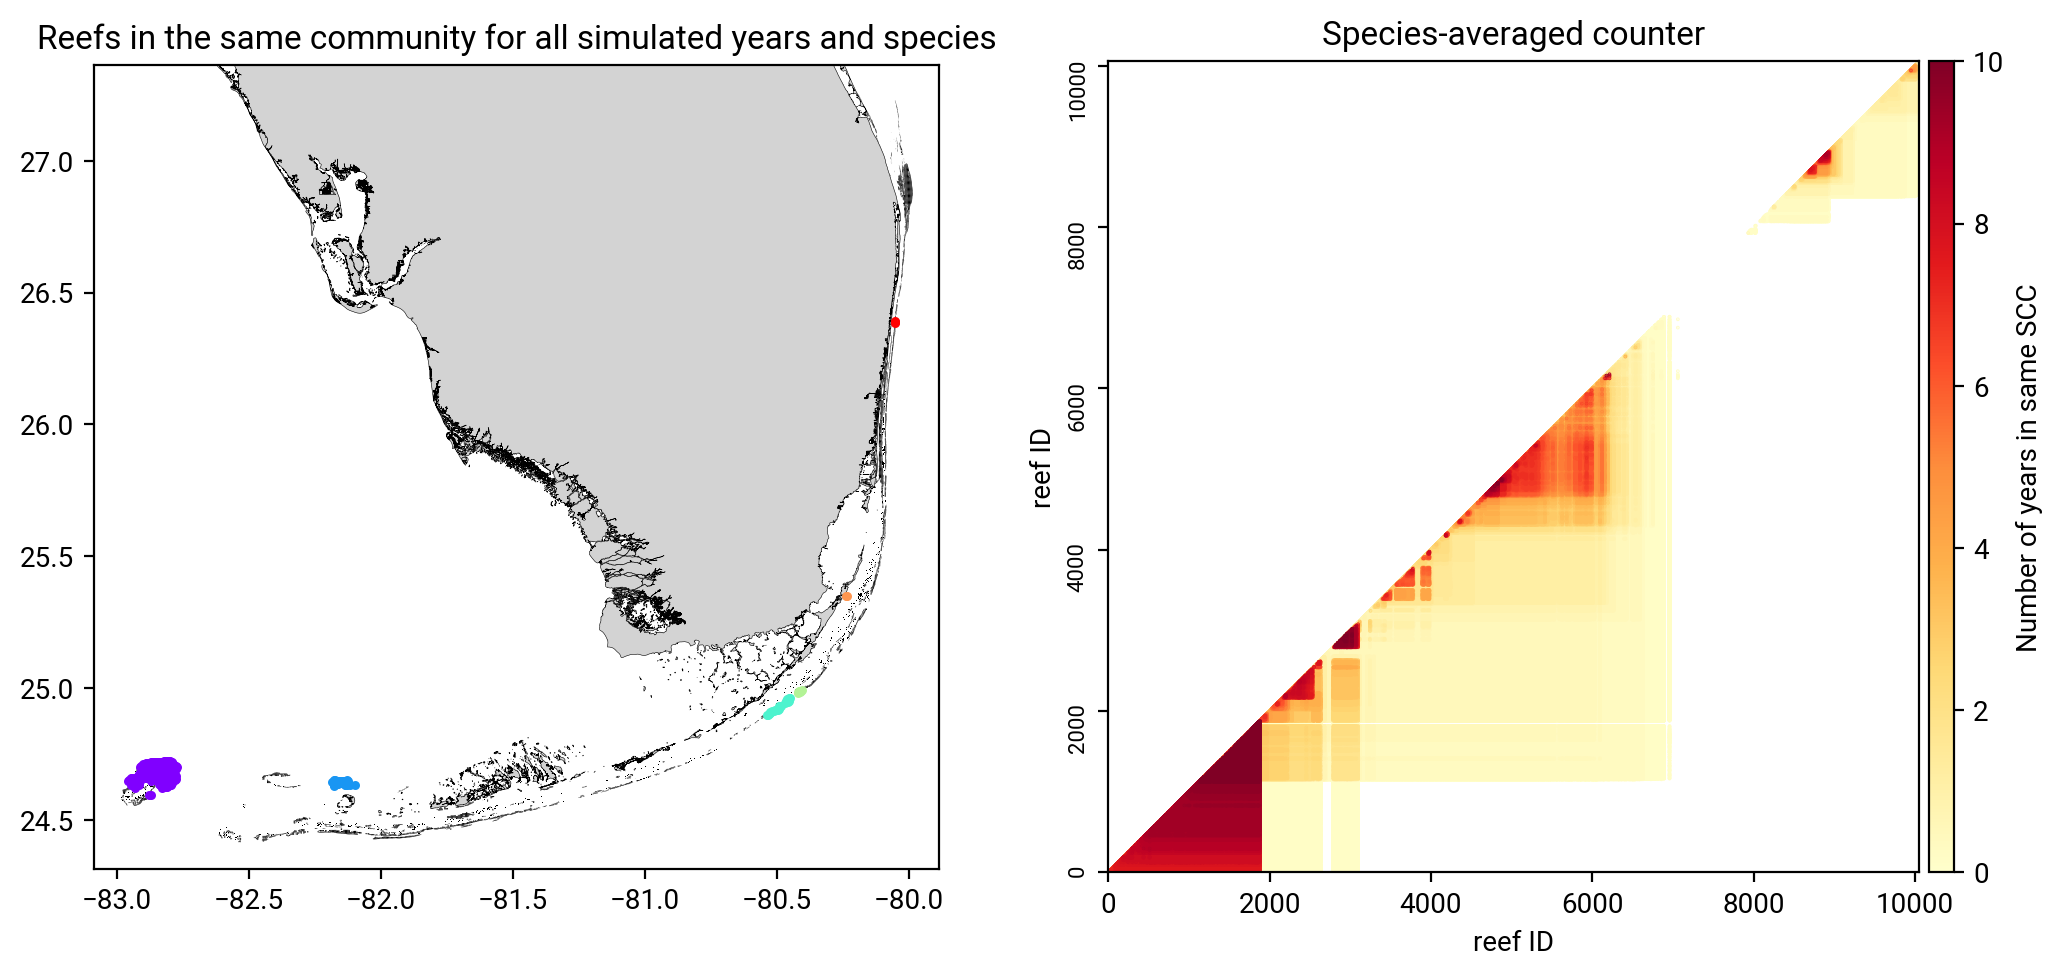
\includegraphics[width=\textwidth]{figures/mean_counter.png}
		\caption{\textbf{Left:} Invariant community made up of reefs found in the same SCC for all simulated years and species. \textbf{Right:} Species-avearged symmetrical matrix total number of simulated years spent by each pair of reefs in the same SCC in the connectivity networks. Reefs are ordered based on their geographical coordinates. Entries of the bottom left (resp. top right) of the matrix correspond to reefs located in the south-west (resp. north-east) of FCR.}\label{fig:mean_counter}
	\end{figure}
	
	
	% === Larval survival and competency measurements === %
	\section{Larval survival and competency measurements and models}\label{appendix:larvae}
	
	\begin{table}
		\centering
		\renewcommand{\arraystretch}{1.5}
		\begin{tabular}{|l|l|}
			\hline
			\textbf{Larval trait} & \textbf{Equation} \\
			\hline
			Mortality (exponential) & $\mu() = \lambda$ \\
			\hline
			Mortality (Weibull): & $\mu(t) = \lambda\nu(\lambda t)^{\nu-1}$ \\
			\hline
			Competency acquisition &  $\renewcommand{\arraystretch}{1}\alpha(t) = \left\{
			\begin{array}{ll}
				0 & t < t_c, \\
				a & \text{otherwise.}
			\end{array}
			\right.$\\
			\hline
			Competency loss & $\beta(t) = b$ \\
			\hline
		\end{tabular}
		\caption{Parameterization of the mortality, competency acquisition and competency loss rates used in the model.}\label{tab:appendix}
	\end{table}
	
	\begin{figure}
		\centering
		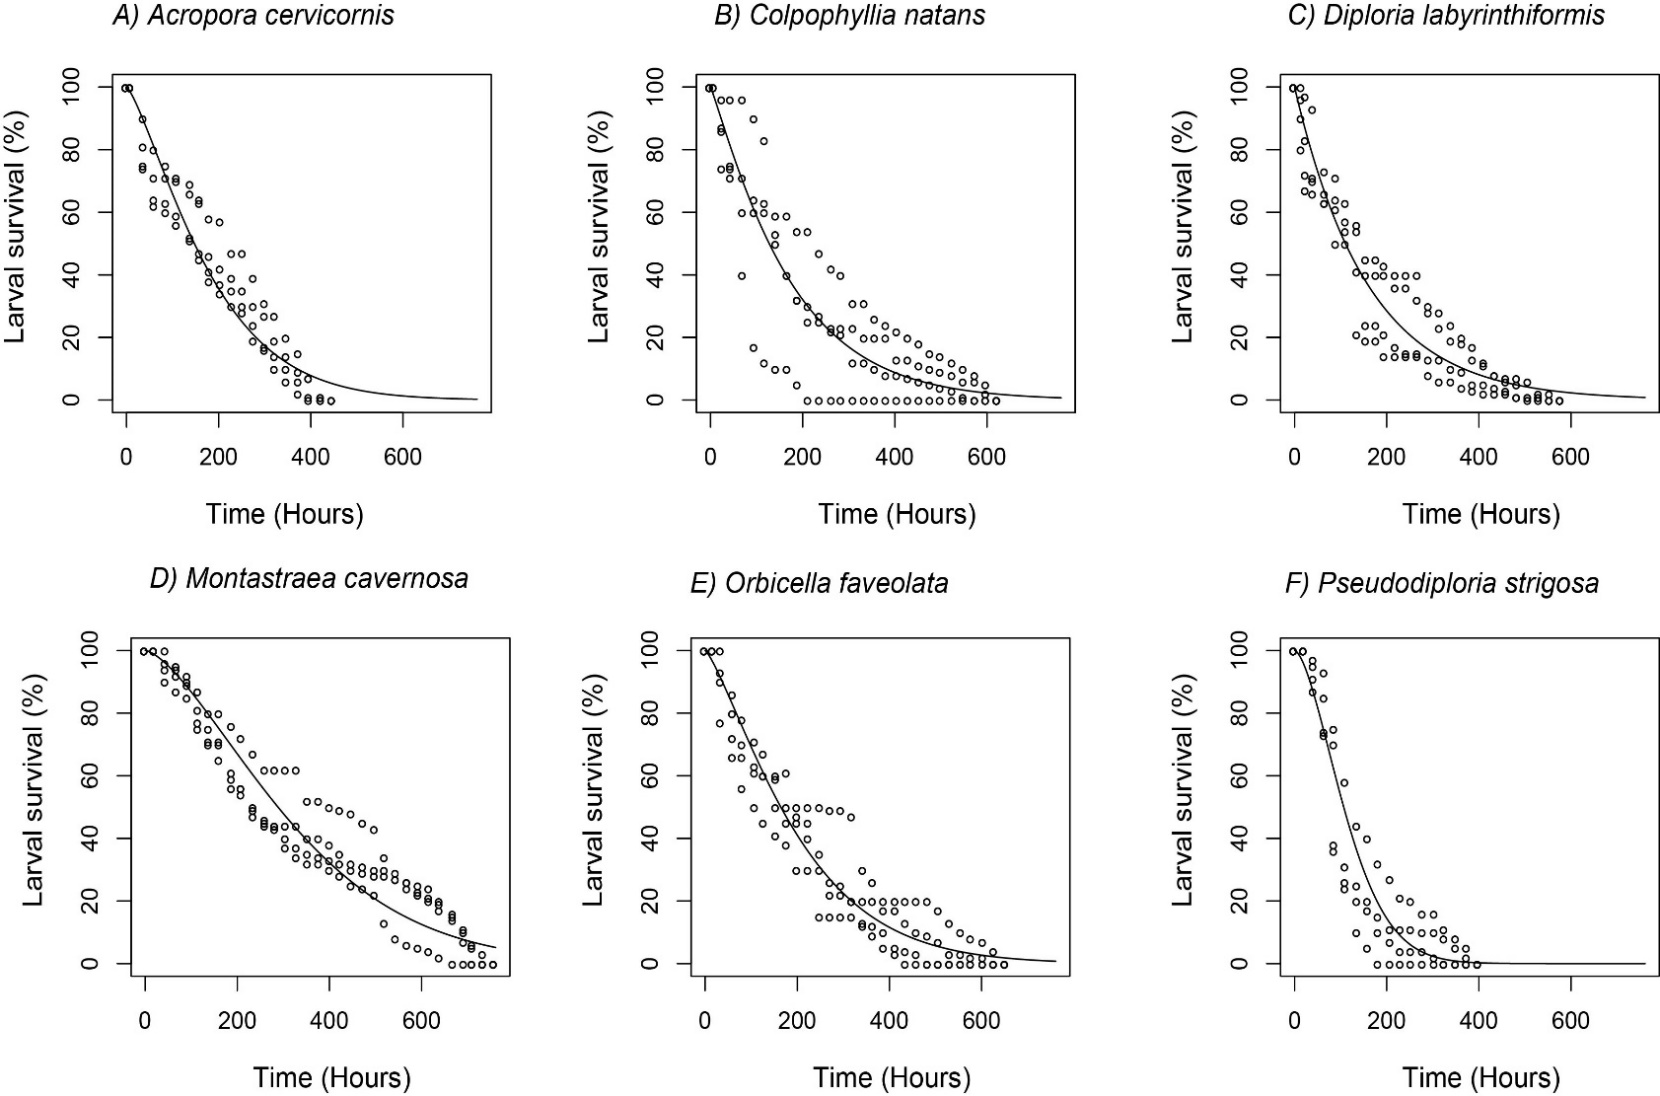
\includegraphics[width=\textwidth]{figures/fig_mortality.jpeg}
		\caption{ Percent larvae alive over time for the six Caribbean coral species studied. A) \textit{A.~cervicornis}, B) \textit{C.~natans}, C) \textit{D.~labyrinthiformis}, D) \textit{M.~cavernosa}, E) \textit{O.~faveolata}, and F) \textit{P.~strigosa}. Circles represent the observations, and lines the best fitted model. The model of best fit for shape of mortality of all species was the standard Weibull model except for \textit{D.~labyrinthiformis}, which mortality was best fit with an exponential model}\label{fig:mortality}
	\end{figure}
	\begin{figure}
		\centering
		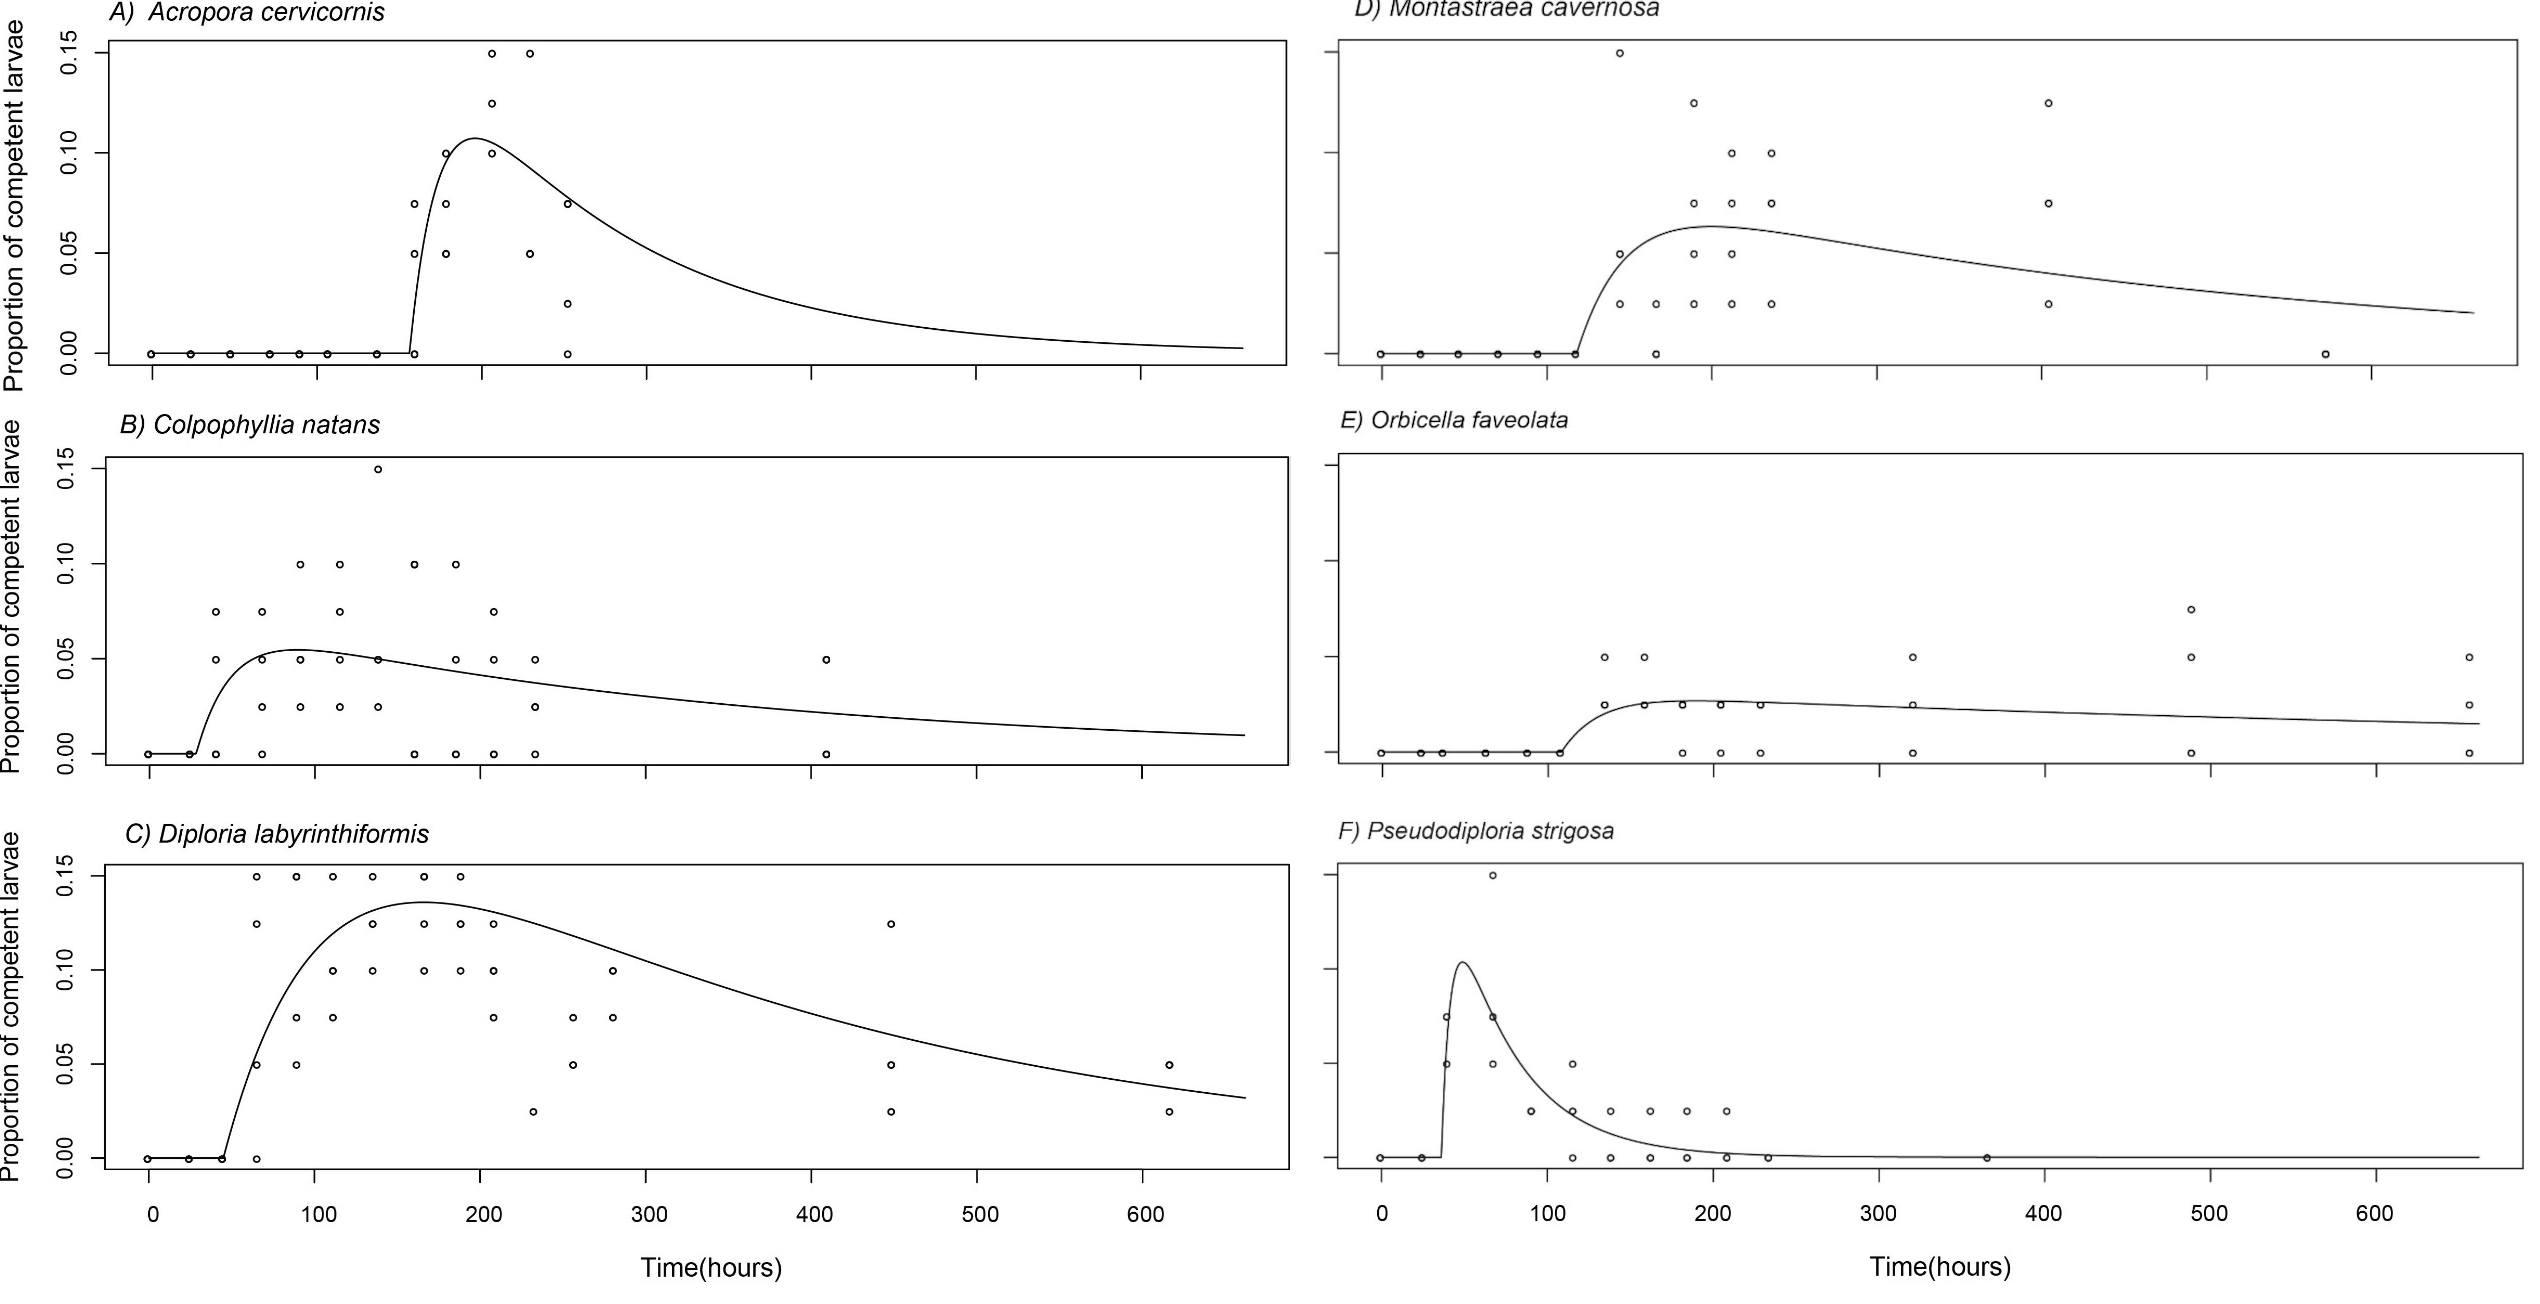
\includegraphics[width=\textwidth]{figures/fig_competence.png}
		\caption{Proportion of competent larvae over time for the six species studied. A) \textit{A.~cervicornis}, B) \textit{C.~natans}, C) \textit{D.~labyrinthiformis}, D) \textit{M.~cavernosa}, E) \textit{O.~faveolata}, and F) \textit{P.~strigosa}. The model of best fit for shape of loss of competency of all species was the exponential model.}\label{fig:competence}
	\end{figure}
	
	\subsection{Methods}
	\subsubsection{Species}

	Through successful induction coral spawning ex situ at Nova Southeastern University, Florida Aquarium, and University of North Carolina Wilmington, we were able to obtain embryos of six coral species, \textit{Diploria labyrinthiformis}, \textit{Acropora cervicornis}, \textit{Pseudodiploria strigosa}, \textit{Colpophyllia natans}, \textit{Montastraea cavernosa}, and \textit{Orbicella faveolata}. 

	\subsubsection{Ex situ coral spawning}
	\textit{Montastraea cavernosa} was the only gonochoric species studied. Sperm was collected using a 25 mL pipette, ensuring the necessary higher concentration of sperm for fertilization \citep{fogarty2012weak, fogarty2012asymmetric, dela2020optimising}. Eggs were collected at the surface of the water and mixed with the sperm in bowls for fertilization. All the other species were hermaphroditic and thus released both eggs and sperm in bundles. Bundles were collected at the surface of the water and put into fertilization bowls. As bundles dissociated, seawater was added to the bowls to attain the sperm concentration close to 106 sperm cells/mL known to maximize fertilization \citep{fogarty2012weak, fogarty2012asymmetric, dela2020optimising}. Fertilization success was confirmed about one to one and a half hours after pooling the gametes by observing embryos undergoing cell division. Embryos were then promptly washed two to three times to remove unused sperm, using a gravy separator to ensure a clean culture. Acropora cervicornis gametes were collected from colonies which sexually matured on the reefs off Fort Lauderdale, FL (USA), and brought to the outdoor aquaria for spawning a few days before their expected spawning time. Orbicella faveolata gametes were obtained from colonies at Biscayne Bay National Park. The other species were kept in aquaria year-round and induced to mature their gonads and spawn in the lab by mimicking natural cycles of light and temperature.

	\subsubsection{Larval survival trials}
	After confirmation of fertilization, 400 fertilized embryos were collected and randomly assigned to one of four separate 200 mL glass jars each containing 100 embryos. Jars were kept on a water bath equipped with a thermostat and a small circulation pump to maintain temperature constant at 28°C. Salinity and temperature were monitored and maintained daily. All larvae were counted daily under a microscope to record the proportion of larvae alive over time. Every day for each species, water in the jar was exchanged and larvae were washed using clean seawater and placed into a clean jar. Survival experiments ended once all larvae had died. 

	\subsubsection{Larval competency trials}
	Once the larvae of each species were observed rotating, \textit{ca.} $3,500$ larvae were randomly divided into three bowls. Bowls were kept in a water bath equipped with a thermostat and a small circulation pump to maintain temperature constant at $28^\circ$C and monitored daily. Aeration was added to each individual bowl to prevent settlement within the bowl and avoid anoxic conditions. The larvae in the bowls were washed daily over a filter using clean seawater. After washing, larvae were placed into clean bowls in the water bath. Daily, 40 larvae from each species were collected at random and divided evenly into four separate 200 mL glass jars that contained one pre-conditioned aragonite tile that had crustose coralline algae sprinkled upon it. After 24 hours, the tile in each jar was examined under the microscope to assess the number of larvae that had settled and metamorphosed. This process was repeated daily; larvae that remained swimming at the end of each day were not reused in the competency trials. Competency trials were completed once all larvae of a species had died in the survival trials. 

	\subsubsection{Modeling}
	Larval survival and competency dynamics for each species were modelled using the methodology described by \cite{figueiredo2022global}. Specifically, in our model, larvae suffer mortality at stochastic rate $\mu(t)$, where $t$ denotes time after spawning. Larvae acquire competence at stochastic rate $\alpha(t)$ and lose competence at stochastic rate $\beta(t)$. Since the survival and competence data sets were collected separately, survival and competence modelling was also performed separately.

	\subsubsection{Survival}
	We used a standard likelihood formulation for our survival analysis. Since no larvae were removed during the study, and larvae were censused at fixed points in time, our design was interval-censored. Thus, the log-likelihood is:
	\begin{equation}
		\log L = \sum_{t=0}^{t_f} \left((A(t-1)-A(t))\log(P_a(t-1)-P_a(t))\right) + A(t_f)\log(P_a(t_f))
	\end{equation}
	where $t$ is time (days since fertilization), $t_f$ is the last day larvae were censused, $A(t)$ is the number of individuals alive at time $t$, $A(t-1)-A(t)$ is the number of larvae that died from one day to the next (i.e. between time $t-1$ and $t$),  $P_a(t)$ is the probability of being alive at time $t$, and $P_a(t-1)-P_a(t)$ is the probability to dying from one day to next (\textit{i.e.} between time $t-1$ and $t$). The probability of being alive at time t is given by:

	\begin{equation}
		P_a(t) = \exp\left(-\int_0^t\mu(\omega)d\omega\right)
	\end{equation}

	For mortality, we considered the standard Weibull survival model, which allows monotonic increases or decreases in mortality rate over time, is the limiting case of the generalized Weibull as $\nu = 0$ (Table \ref{tab:appendix}), and the exponential model, according to which mortality rate is constant over time, is the special case of the Weibull model when $\nu=1$ (Table \ref{tab:appendix}). To assess which distribution (exponential or Weibull) best described the survival dynamics, we fitted the survival data to the two possible distributions, estimating the parameters with maximum likelihood methods and using AICc (Akaike’s Information Criterion with the small-sample bias-correction term) to select the model that best described the survival dynamics. 
	\subsubsection{Competence}
	For the acquisition of competence, since there is a minimum period of time required for individuals to complete embryogenesis and develop the structures needed for settlement, we assume that $\alpha(t) = 0$ when $t < t_c$  and afterwards larvae acquire competence at a constant stochastic rate $a$ (Table \ref{tab:appendix}). After acquiring competence, larvae lose competence at a stochastic rate $\beta(t)$ which was constant over time, \textit{i.e.} was well fit with an exponential distribution, thus $\beta(t) =b$. The competence likelihood is given by the probability of being competent at each of the sampling days ($t$), which is given by the probability density of having acquired competence between time $t_c$, and $t$, and remained competent until at least time t:

	\begin{equation}
		P_c(t)=\int_{t_c}^t a\exp\left(-a(\tau-t_c) - \int_0^{t-\tau}\beta(\gamma)d\gamma\right)d\tau
	\end{equation}

	\subsection{Results}
	In the absence of settlement cues, larval survival decreased over time for all species, with \mcav displaying the lowest and \pstr displaying the highest mortality rates (Figure \ref{fig:mortality}). The per capita mortality rate was constant over time for \textit{D.~labyrinthiformis}, but decreased over time for all the other species i.e., was higher during embryogenesis (likely because defective cell-divisions are more fatal) than once most larvae had reached the planula stage (2-7 days after spawning). It remains to be determined if the recorded rates of larval mortality are species-specific and/or driven by parental genotype, history of stress exposure, and food quantity and quality they had access to, and/or symbiont community \citep{jones2011tradeoffs, baums2013genotypic,padilla2013all,kirk2018genomic}.

	The estimated rates of acquisition (a) and loss of competency (b) also differed between species (Table \ref{tab:appendix}, Figure \ref{fig:competence}). For some species, the percentage of larvae that settled was quite low, thus is possible that the crustose coralline algae and microbial biofilm used to induce settlement were not as adequate for them. However, the species that displayed lower settlement, \textit{P.~strigosa}, also registered the highest mortality suggesting that rather than species-specific, rates of mortality, and acquisition and loss of competency are mostly explained by parental condition. Furthermore, because larvae lose competency when they exhaust their energy reserves, species with larger eggs, \ie theoretically more energy reserves, were hypothesized to remain competent for longer periods of time, but this is not supported by our data. The rate of loss competency might instead be related to the quality of those energy reserves. It is also possible that species with larger eggs have higher metabolic rates and thus exhaust their energy disproportionally faster. The interspecific differences in the minimum time to competency are unequivocally species-specific, and likely explained by egg size \citep{figueiredo2025predicting}.
%

\end{document}
\endinput
